{\pdfoutput=1
\documentclass[runningheads,a4paper]{llncs}

\usepackage{amssymb}
\usepackage{amsmath}
\setcounter{tocdepth}{3}
\usepackage{graphicx}
\usepackage{amsmath}
\usepackage{hyperref}
\usepackage{todonotes}
\usepackage{datetime}
\usepackage{listings}
\usepackage{xcolor}
\usepackage{wrapfig}
\usepackage{subfig}
\usepackage{booktabs}
\usepackage{url}
\usepackage{float}

\renewcommand{\arraystretch}{1.3}

\newcommand{\todonoteinline}[1]{\todo[color=red!40,inline,caption={TODO}]{#1}}
\newcommand{\todonote}[1]{\todo[color=red!40,caption={TODO}]{#1}}

\newcommand{\nonmetrlib}{Non-Metric Space Library}
\newcommand{\replocdir}{https://github.com/searchivarius/NonMetricSpaceLib/tree/master/}
\newcommand{\replocfile}{https://github.com/searchivarius/NonMetricSpaceLib/blob/master/}
\newcommand{\ttt}[1]{\texttt{#1}}
\newcommand{\knn}{$k$-NN }
\newcommand{\knnns}{$k$-NN}
\newcommand{\ED}{\mbox{\rm ED}}
\newcommand{\pos}{\mbox{\rm pos}}
\newcommand{\rev}{\mbox{\rm rev}}
\newcommand{\DEL}[2]{\Delta_{#1}(#2)}

\setcounter{secnumdepth}{3}

\begin{document}

\mainmatter  % start of an individual contribution

% first the title is needed
\title{\nonmetrlib{} Manual}

% a short form should be given in case it is too long for the running head
\titlerunning{\nonmetrlib{} Manual}

% the name(s) of the author(s) follow(s) next
%
% NB: Chinese authors should write their first names(s) in front of
% their surnames. This ensures that the names appear correctly in
% the running heads and the author index.
%
\author{Bilegsaikhan Naidan\inst{1} \and Leonid Boytsov\inst{2}}
%
\authorrunning{Bilegsaikhan Naidan and Leonid Boytsov}
% (feature abused for this document to repeat the title also on left hand pages)

% the affiliations are given next; don't give your e-mail address
% unless you accept that it will be published
\institute{
Department of Computer and Information Science,\\
Norwegian University of Science and Technology,\\
Trondheim, Norway\\
{\hspace{1em}}\\
\and
Language Technologies Institute, \\
Carnegie Mellon University,\\
Pittsburgh, PA, USA\\
\email{srchvrs@cs.cmu.edu}\\
}

%
% NB: a more complex sample for affiliations and the mapping to the
% corresponding authors can be found in the file "llncs.dem"
% (search for the string "\mainmatter" where a contribution starts).
% "llncs.dem" accompanies the document class "llncs.cls".
%

%\toctitle{Lecture Notes in Computer Science}
%\tocauthor{Authors' Instructions}

\maketitle

{\begin{center}{\small \textbf{Maintainer}: Leonid Boytsov}\end{center}}
{\begin{center}{Version 1.0}\end{center} 
{\begin{center}{{\today}}\end{center}}

\begin{abstract}
This document describes a library for similarity searching.
Even though the library contains a variety of metric-space access methods,
our main focus is on search methods for non-metric spaces.
Because there are fewer exact solutions for non-metric spaces,
many of our methods give only approximate answers. 
Thus, the methods
are evaluated in terms of efficiency-effectiveness trade-offs
rather than merely in terms of their efficiency.
Our goal is, therefore, to provide
not only state-of-the-art approximate search methods for 
both non-metric and metric spaces,
but also the tools to measure search quality.
We concentrate on technical details, i.e., 
how to compile the code, run the benchmarks, evaluate results,
and use our code in other applications.
Additionally, we explain how to extend the code by adding
new search methods and spaces.
\end{abstract}

\section{Introduction}
\subsection{Motivation}
The Non-Metric Space Library is a collection of
similarity search methods and a toolkit for their evaluation.
Our software suit can also be used as a standalone search library on Linux and Windows. 
Most search methods were implemented by Bileg(saikhan) Naidan and Leo(nid) Boytsov.\footnote{Leo(nid) Boytsov is a maintainer.}
Additional contributors are listed on the \href{https://github.com/searchivarius/NonMetricSpaceLib}{GitHub 
page}.
%We encourage potential users and contributors to use GitHub for bug reports.

The code written by Bileg and Leo is distributed under the business-friendly \href{http://apache.org/licenses/LICENSE-2.0}{Apache License}. 
Some contributions are licensed differently.
For more information regarding licensing and acknowledging the use of the library
resource, please refer to \S~\ref{SectionCredits}.

The design of the library was influenced by 
and superficially resembles the design of the Metric Spaces Library \cite{LibMetricSpace}.
Yet our approach is different in many ways:

\begin{itemize}
\item We focus on approximate\footnote{
An approximate method may not
return a true nearest-neighbor or
 all the points within a given query ball.}
  search methods and non-metric spaces.

\item We simplify experimentation, in particular, 
through automatically measuring and aggregating important parameters
related to speed and accuracy. 
In addition, we provide capabilities for testing in both single- and multi-threaded modes
to ensure that implemented solutions scale well with the number of available CPUs.

\item We care about overall efficiency and
aim to implement methods that have runtime comparable to an optimized production system. 
\end{itemize}

Search methods for non-metric spaces are especially interesting.
This domain does not provide sufficiently generic \emph{exact} search methods.
We may know very little about analytical properties of the distance
or the analytical representation may not be available at all (e.g., if the 
distance is computed by a black-box device \cite{Skopal:2007}).
In many cases it is not possible to search exactly
and instead one has to resort to approximate search procedures.

This is why methods
are evaluated in terms of efficiency-effectiveness trade-offs
rather than merely in terms of their efficiency.
We believe that there is no ``one-size-fits-all'' search method.
Hence, it is important to being able to evaluate the ``goodness of fit''
for a particular  domain.

Our commitment to efficiency affected several design decisions:
\begin{itemize}
\item The library is implemented in C++;
\item We focus on in-memory indices 
and, thus, do not require our methods to materialize a disk-based version of an index
(this also reduces programming effort).
It is, nevertheless, possible to benchmark disk-based implementations as well (see \ref{SectionWorkflow}).

\item 
We provide efficient implementations of many distance functions,
which rely on Single Instruction Multiple Data (SIMD) CPU commands  and/or
approximation of computationally intensive mathematical operations (see \S~\ref{SectionEfficiency}). 
\end{itemize}

It is often possible to demonstrate a substantial reduction in the number of distance computations
compared to sequential searching.
However, such reductions entail additional computations (i.e., extra book-keeping)
and do not always lead to improved overall performance \cite{Boytsov_and_Bilegsaikhan:sisap2013}.
To eliminate situations where book-keeping costs are ``masked''
by inefficiencies of the distance function,
we pay special attention to distance function efficiency.

\subsection{Problem Formulation}
Similarity search is an essential part of many applications,
which include, among others,  
content-based retrieval of multimedia  and statistical machine learning.
The search is carried out on a finite database of objects $\{o_i\}$ (we also used a term data point or simply point),
using a search query $q$ and a dissimilarity measure.
The dissimilarity measure is typically represented by a distance function $d(o_i, q)$. 
The ultimate goal is to answer a query by retrieving a subset of database objects sufficiently similar to the query $q$.
These objects will be called \ttt{answers}.
Note that we use the terms \ttt{distance} and the \ttt{distance function} in a broader sense:
We do not assume that the distance is a true metric distance. 
The distance can be asymmetric and is not constrained to be metric (i.e., 
it may not satisfy the triangle inequality).

Two retrieval tasks are typically considered: a nearest neighbor and a range search. 
The nearest neighbor search aims to find the least dissimilar object,
i.e., the object at the smallest distance from the query.
Its direct generalization is the $k$-nearest neighbor search (the \knn search),
which looks for the $k$ most closest objects.
Given a radius $r$, 
the range query retrieves all objects within a query ball (centered at the query object $q$) with the radius $r$,
or, formally, all the objects~$\lbrace o_i \rbrace$ such that $d(o_i, q) \le r$. 
In generic spaces, the distance is not necessarily symmetric. 
Thus, two types of queries can be considered. 
In a  \emph{left} query, the object is the left argument of the distance function,
while the query is the right argument.
In a \emph{right} query, $q$ is the first argument and the object is the second, i.e.,
the right, argument.

The queries can be answered either exactly, 
i.e., by returning a complete result set that does not contain erroneous elements, or, 
approximately, e.g., by finding only some answers.
Thus, the methods are evaluated in terms of efficiency-effectiveness trade-offs
rather than merely in terms of their efficiency.
One common effectiveness metric is recall. In the case
of the nearest neighbor search, it is computed as
an average fraction of true neighbors returned by the method.
If ground-truth judgements (produced by humans) are available,
it is possible to compute an accuracy of a \knn based classification
(see \S~\ref{SectionEffect}).

In the current release, we focus on vector-space implementations,
i.e., all the distance functions are defined over real-valued vectors. 
Note that this is not a principal limitation, 
because most methods do not access data objects
directly. 
Instead, they rely only on distance values.
In the future, we plan to add more complex spaces, in particular, string-based.

\section{Getting Started}
\subsection{Prerequisites}
The Non-Metric Space Library was developed and tested on 64-bit Linux.
Yet, almost all the code (except LSHKIT) can be built and run on 64-bit Windows.
Building the code requires a modern C++ compiler that supports \mbox{C++11}.
Currently, we support GNU C++ ($\ge4.7$), Intel compiler ($\ge14$), 
Clang ($\ge4.2.1$), 
and Visual Studio ($\ge12$). 
Under Linux, the build process relies on CMake. 
Under Windows, one can use Visual Studio projects stored in the repository.

Note, however, that we do not have a portable code to measure memory consumption:
This part will work only for Linux (with \href{https://en.wikipedia.org/wiki/Procfs}{PROCFS})
and Windows. 

More specifically, for Linux we require:
\begin{enumerate}
\item A \textbf{64-bit} distributive (Ubuntu \textbf{LTS} is recommended);
\item GNU C++ ($\ge4.7$), Intel Compiler ($\ge14$), Clang ($\ge4.2.1$);
\item Cmake (GNU make is also required);
\item Boost (dev version $\ge48$, Ubuntu package \ttt{libboost1.48-all-dev});
\item GNU scientific library (dev version, Ubuntu package \ttt{libgsl0-dev}).
\end{enumerate}

For Windows, we require:
\begin{enumerate}
\item A \textbf{64-bit} distributive (we tested on Windows 8); 
\item Visual Studio Express (or Professional) version 12 or later;
\item Boost is not required to build the core library and unit tests, 
but it is needed by the main testing binary (see \S~\ref{SectionBuildWindows}). 
\end{enumerate}

Efficient implementations of many distance functions (see \S~\ref{SectionEfficiency})
rely on SIMD instructions,
which operate on small  vectors of integer of floating point numbers. 
These instructions are available on most modern processors,
but we support only SIMD instructions available on recent Intel and AMD processors.   
Each distance function has a pure C++ implementation,
which can be less efficient than an optimized SIMD-based implementation.
On Linux, SIMD-based implementations are activated automatically 
for all sufficiently recent CPUs. On Windows, it is necessary to update
project settings manually (see \S\ref{SectionBuildWindows}).

Scripts to generate and process data sets are written in Python.
We also provide the Python script to plot performance graphs: \href{\replocfile sample_scripts/sample_scripts/genplot.py}{genplot.py} (see \S~\ref{SectionGenPlot}).
In addition to Python, this plotting script requires Latex and PGF. 

\subsection{Installing C++11 Compilers}
Installing C++11 compilers can be tricky, 
because they are not always provided as a standard package.
This is why we briefly review the installation process here. 

It is, perhaps, the easiest to obtain Visual Studio 12 by simply downloading
it from the \href{http://www.microsoft.com/en-us/download/details.aspx?id=40787}{Microsoft 
web-page}.
We were able to build and run the 64-bit code using the free distributive of Visual Studio Express 12 (also called 
\ttt{Express 2013}). The professional (and expensive) version of Visual Studio is not required. 


To install GNU C++ version 4.7 on some Linux distributions with the Debian package management system, 
one can simply type:
\begin{verbatim}
sudo apt-get install gcc-4.7 g++-4.7
\end{verbatim}
However, it did not work for us and we needed to use an experimental repository as follows:
\begin{verbatim}
sudo add-apt-repository ppa:ubuntu-toolchain-r/test
sudo apt-get update
sudo apt-get install gcc-4.7 g++-4.7
\end{verbatim}
If the script \ttt{add-apt-repository} is missing, it can be installed as follows:
\begin{verbatim}
sudo apt-get install python-software-properties
\end{verbatim}
More details can be found on the \href{http://askubuntu.com/questions/113291/how-do-i-install-gcc-4-7}{AskUbuntu web-site.}

Similarly to the GNU C++ compiler, to install a C++11 version of Clang, one may need to add a non-standard repository.
For Debian and Ubuntu distributions, it is easiest to add repositories from \href{http://llvm.org/apt/}{
the LLVM web-site}. For example, if you have Ubuntu 12 (Precise), you need to add repositories
as follows:\footnote{Do not forget to remove \ttt{deb-src} for source repositories.
See the discussion \href{http://askubuntu.com/questions/160511/why-does-add-apt-repository-fail-to-add-source-repositories}{here for more details.}}
\begin{verbatim}
sudo add-apt-repository \
  "deb http://llvm.org/apt/precise/ llvm-toolchain-precise main"
sudo add-apt-repository \
  "http://llvm.org/apt/precise/ llvm-toolchain-precise main"
sudo add-apt-repository \
  "deb http://llvm.org/apt/precise/ llvm-toolchain-precise-3.4 main"
sudo add-apt-repository \
  "http://llvm.org/apt/precise/ llvm-toolchain-precise-3.4 main"
sudo add-apt-repository \
  "deb http://ppa.launchpad.net/ubuntu-toolchain-r/test/ubuntu \
                                                  precise main"
\end{verbatim}
Then, Clang 3.4 (and LLDB debugger) can be installed by typing:
\begin{verbatim}
sudo apt-get install clang-3.4 lldb-3.4
\end{verbatim}

The Intel compiler can be freely used for non-commerical purposes.
It is a part of C++ Composer XE for Linux and can 
be obtained \href{http://software.intel.com/en-us/non-commercial-software-development}{from the Intel web site}.
After downloading and running an installation script, one needs to set environment variables.
If the compiler is installed to the folder \ttt{/opt/intel}, environment variables
are set by a script as follows:
\begin{verbatim}
/opt/intel/bin/compilervars.sh intel64
\end{verbatim}

One pitfall on Linux is that installing compilers does 
not necessarily make them default compilers.
One way to fix this is to set environment variables \ttt{CXX} and \ttt{CC}.
For the GNU 4.7 compiler:
\begin{verbatim}
export CXX=g++-4.7 CC=gcc-4.7 
\end{verbatim}
For the Clang compiler:
\begin{verbatim}
export CXX=clang++ CC=clang
\end{verbatim}
For the Intel compiler:
\begin{verbatim}
export CXX=icc CC=icc 
\end{verbatim}


\subsection{Quick Start on Linux}\label{QuickStartLinux}
To build the project, go to the directory \href{\replocdir similarity_search}{similarity\_search} and type:  
\begin{verbatim}
cmake .  
make   
\end{verbatim}
This creates several binaries in the directory \ttt{similarity\_search/release}, 
most importantly, a semi unit test utiltity \ttt{bunit}
and a benchmarking utility \ttt{experiment}, which carries out experiments.
Examples of using this benchmarking utility can be found in the directory \href{\replocdir sample_scripts}{sample\_scripts}. 
Please, check the script \href{\replocfile sample_scripts/sample_run.sh}{sample\_run.sh}. 

A more detailed description of the build process on Linux is given in \S~\ref{SectionBuildLinux}.

\subsection{Quick Start on Windows}\label{QuickStartWindows}
Building on Windows is straightforward:
One can simply use the provided \href{\replocfile similarity_search/NonMetricSpaceLib.sln}{Visual Studio 
solution file}.
The solution file references several project (*.vcxproj) files: 
\href{\replocfile similarity_search/src/NonMetricSpaceLib.vcxproj}{NonMetricSpaceLib.vcxproj}
is the main project file that is used to build the library itself.
The core library, the semi unit test binary (\ttt{bunit}),
 as well as examples of the standalone applications (projects \ttt{sample\_standalone\_app1}
and \ttt{sample\_standalone\_app2})
can be built without installing Boost. The output is stored in the folder \ttt{similarity\_search\textbackslash x64}.

A more detailed description of the build process on Windows is given in \S~\ref{SectionBuildWindows}.

\section{Building and running the code (in detail)}

A build process creates several important binaries, which include:

\begin{itemize}
\item The \nonmetrlib{} library (on Linux \ttt{libNonMetricSpaceLib.a}),
which can be used in external applications;
\item The main benchmarking utility \ttt{experiment} (\ttt{experiment.exe} on Windows) 
that carries out experiments and saves evaluation results;
\item A tuning utility \ttt{tune\_vptree} (\ttt{tune\_vptree.exe} on Windows) 
that finds optimal VP-tree parameters (see our paper for details \cite{Boytsov_and_Bilegsaikhan:nips2013});
\item A semi unit test utility \ttt{bunit} (\ttt{bunit.exe} on Windows);
\item A utility \ttt{bench\_distfunc} that carries out integration tests (\ttt{bench\_distfunc.exe} on  Windows);
\end{itemize}

A build process is different under Linux and Windows. 
In  the following sections, we consider these differences in more detail. 

\subsection{Building under Linux}\label{SectionBuildLinux}
Implementation of similarity search methods is in the directory \ttt{similarity\_search}.
The code is built using a \ttt{cmake}, which works on top of the GNU make.
Before creating the makefiles, we need to ensure that a right compiler is used.
This is done by setting two environment variables: \ttt{CXX} and \ttt{CC}.
In the case of GNU C++ (version 4.7), you need to type:
\begin{verbatim}
export CCX=g++-4.7 CC=gcc-4.7 
\end{verbatim}
In the case of the Intel compiler, you need to type:
\begin{verbatim}
export CXX=icc CC=icc 
\end{verbatim}


To create makefiles for a release version of the code, type:
\begin{verbatim}
cmake -DCMAKE_BUILD_TYPE=Release .
\end{verbatim}
If you did not create any makefiles before, you can shortcut by typing:
\begin{verbatim}
cmake . 
\end{verbatim}
To create makefiles for a debug version of the code, type:
\begin{verbatim}
cmake -DCMAKE_BUILD_TYPE=Debug .
\end{verbatim}
When makefiles are created, just type:
\begin{verbatim}
make
\end{verbatim}
If the compiler complains about the wrong version of the GCC, 
it is most likely that you forgot to set the environment variables \ttt{CXX} and \ttt{CC} (as described above).
If this is the case, make these variables point to the correction version of the compiler.
\textbf{Important note:} 
do not forget to delete the \ttt{cmake} cache file, before recreating the makefiles:
\begin{verbatim}
rm CMakeCache.txt
\end{verbatim}

Also note that, for some reason, \ttt{cmake} may ignore environmental variables \ttt{CXX} and \ttt{CC}.
Then, you can specify the compiler directly through \ttt{cmake} arguments.
For example, in the case of the GNU C++ and the \ttt{Release} build, 
this can be done as follows:
\begin{verbatim}
cmake -DCMAKE_BUILD_TYPE=Release -DCMAKE_CXX_COMPILER=g++-4.7 \
-DCMAKE_GCC_COMPILER=gcc-4.7 CMAKE_CC_COMPILER=gcc-4.7 .
\end{verbatim} 

The build process creates several binaries. Most importantly,
the main benchmarking utility \ttt{experiment}.
The directory \ttt{similarity\_search/release} contains release versions of
these binaries. Debug versions are placed into the folder \ttt{similarity\_search/debug}.

\textbf{Important note:} a shortcut command:
\begin{verbatim}
cmake .
\end{verbatim} 
(re)-creates makefiles for the previously 
created build. When you type \ttt{cmake .} for the first time,
it creates release makefiles. However, if you create debug
makefiles and then type \ttt{cmake .}, 
this will not lead to creation of release makefiles! 

To use the library in external applications, which do not belong to the library repository,
one needs to install the library first.
Assume that an installation location is the folder \ttt{NonMetrLibRelease} in the
home directory. Then, the following commands do the trick:
\begin{verbatim}
cmake \
    -DCMAKE_INSTALL_PREFIX=$HOME/NonMetrLibRelease \
    -DCMAKE_BUILD_TYPE=Release .
make install
\end{verbatim}

A directory \href{\replocfile sample_standalone_app}{sample\_standalone\_app} 
contains two sample programs (see files 
\href{\replocfile sample_standalone_app/sample_standalone_app1.cc}{sample\_standalone\_app1.cc}
and
\href{\replocfile sample_standalone_app/sample_standalone_app2.cc}{sample\_standalone\_app2.cc})
that use the \nonmetrlib{} installed in the folder \ttt{\$HOME/NonMetrLibRelease}.

\subsubsection{Developing and Debugging on Linux}
There are several debuggers that can be employed.
Among them, some of the most popular are: \ttt{gdb} (a command line tool)
and a \ttt{ddd} (a GUI wrapper for gdb).
For users who prefer IDEs, one good option is Eclipse IDE for C/C++
developers.
It is not the same as Eclipse for Java and one needs 
to \href{http://www.eclipse.org/downloads/moreinfo/c.php}{download 
this version of Eclipse separately.}.

\begin{figure}
\centering
\caption{\label{FigEclipse1}Selecting an existing project to import}
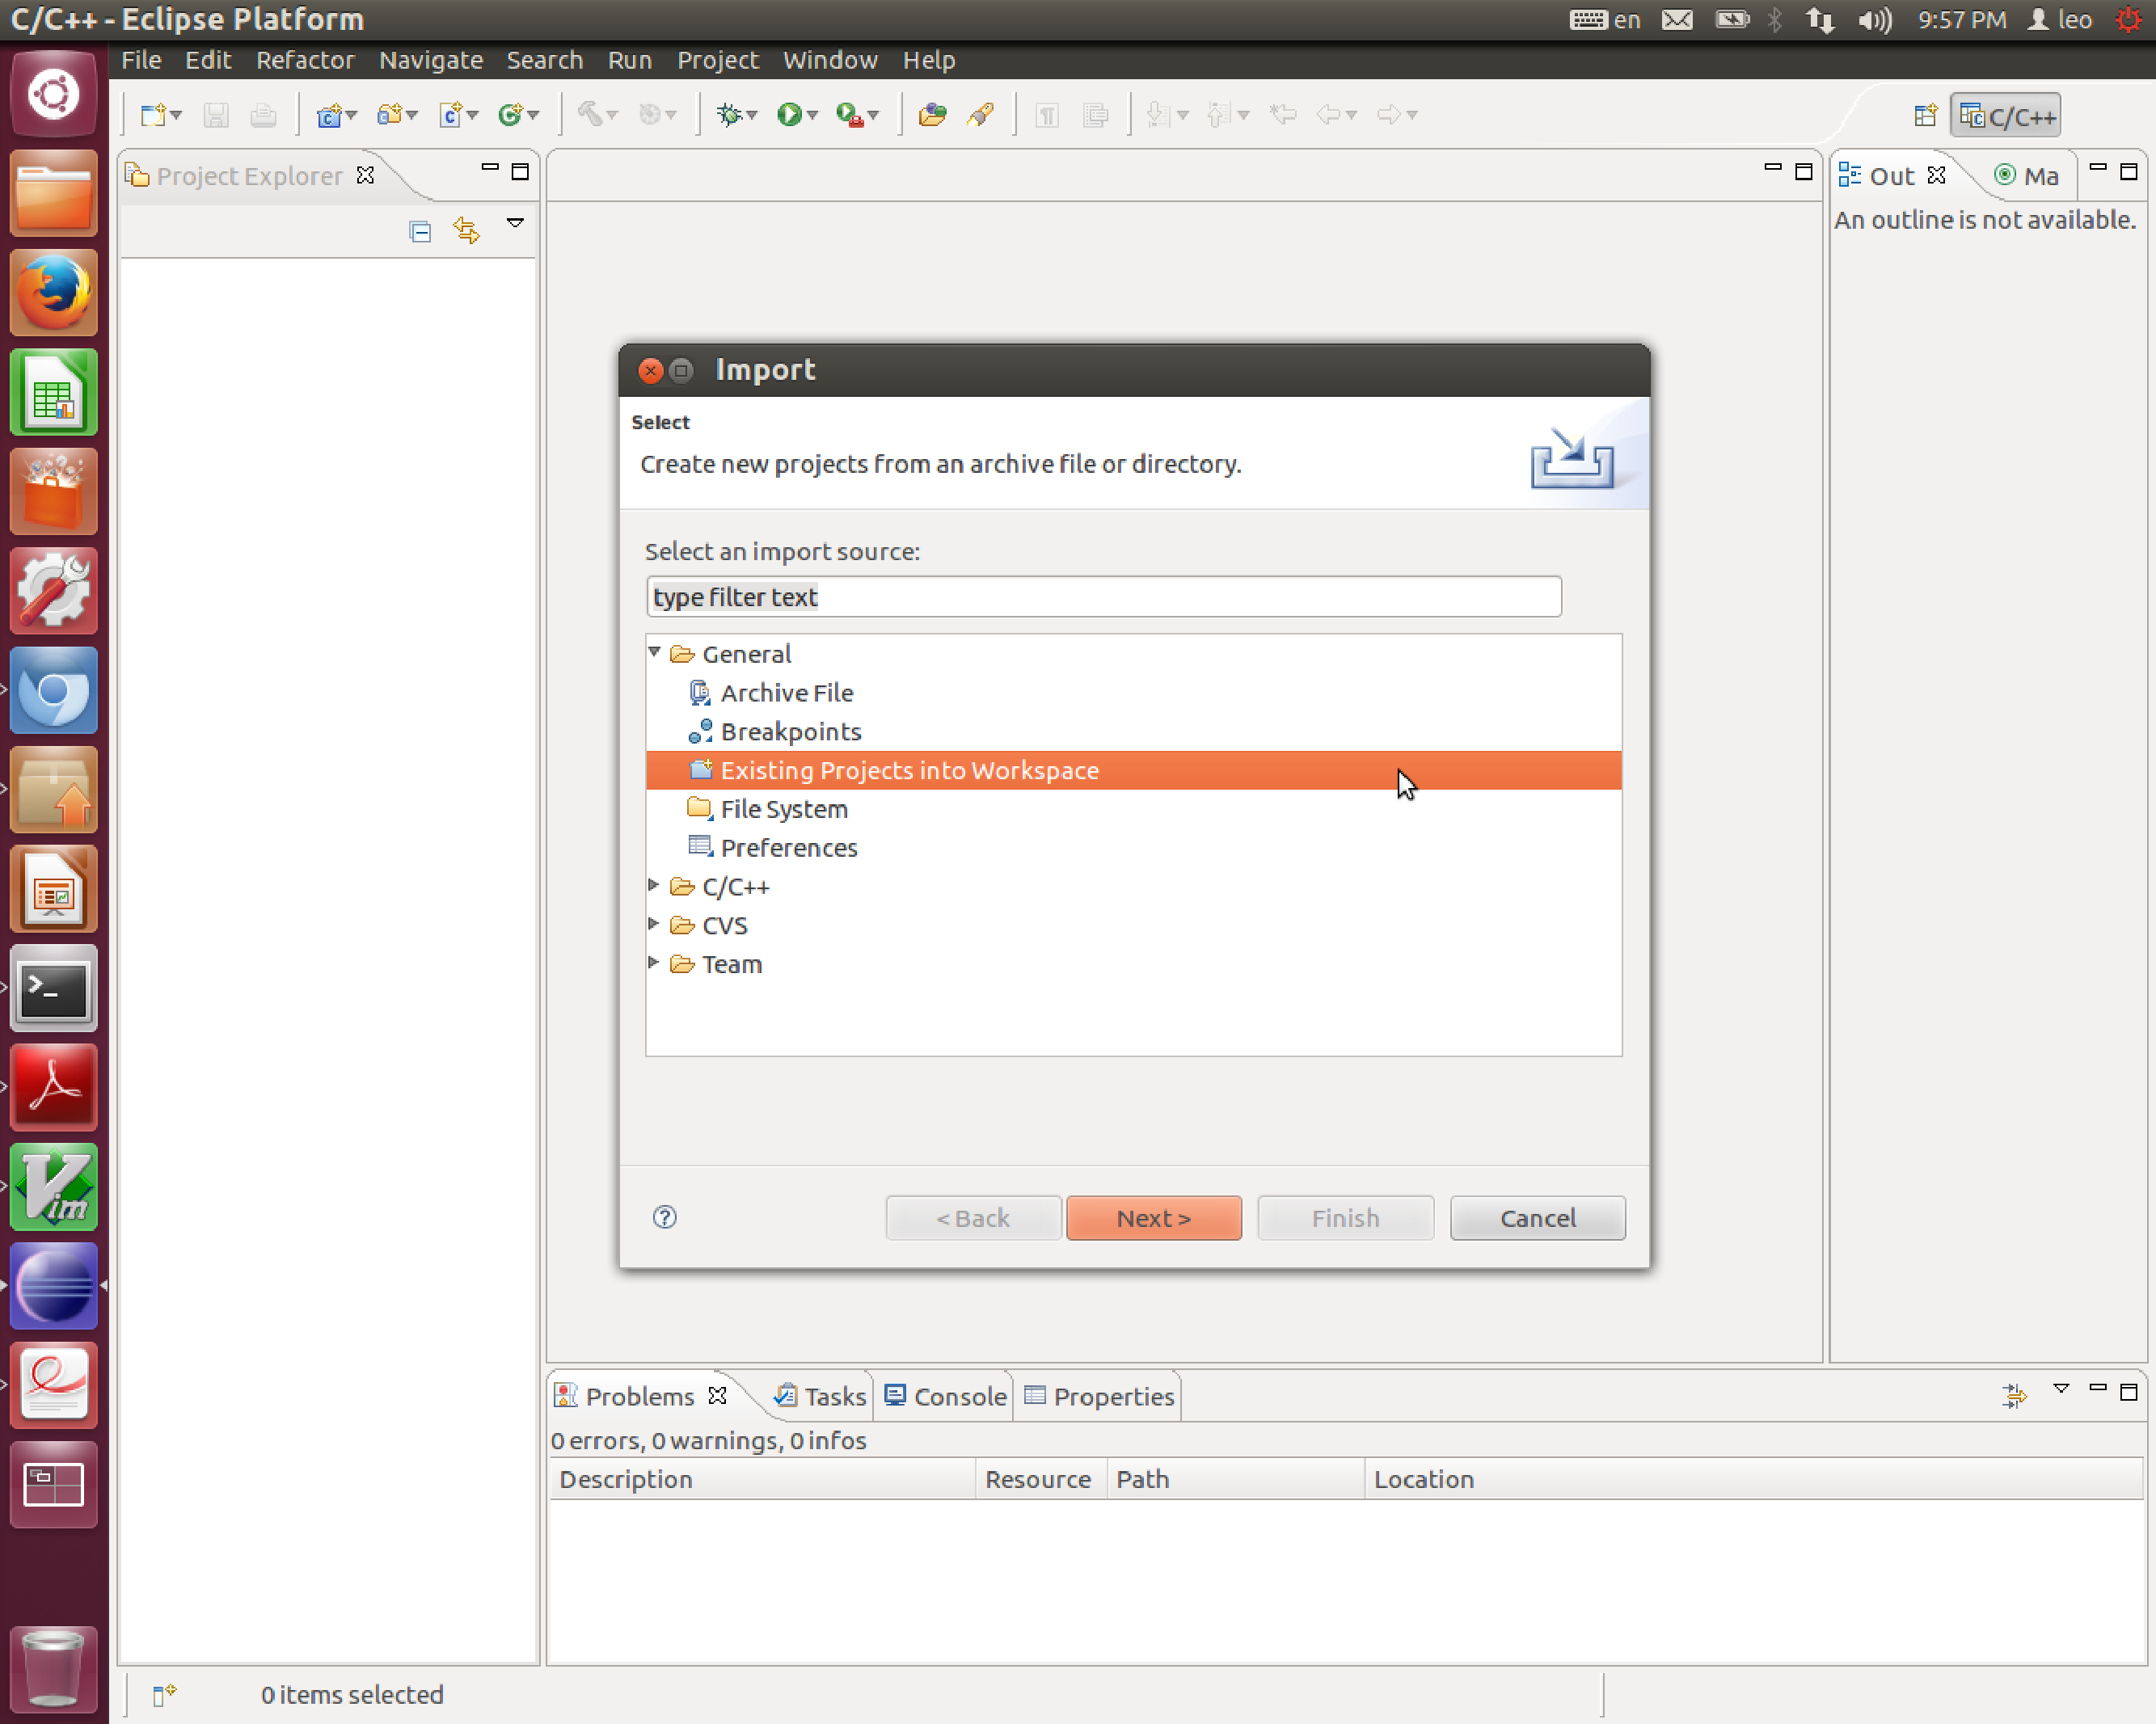
\includegraphics[width=0.9\textwidth]{figures/Eclipse1.pdf}
\end{figure}

After downloading and decompressing, e.g. as follows:
\begin{verbatim}
tar -zxvf eclipse-cpp-europa-winter-linux-gtk-x86_64.tar.gz
\end{verbatim}
one can simply run the binary \ttt{eclipse} (in a
newly created directory \ttt{eclipse}).
On the first start, Eclipse will ask you select a repository location.
This would be the place to store the project metadata and (optionally)
actual project source files.

\begin{figure}
\centering
\caption{\label{FigEclipse2}Importing an existing project}
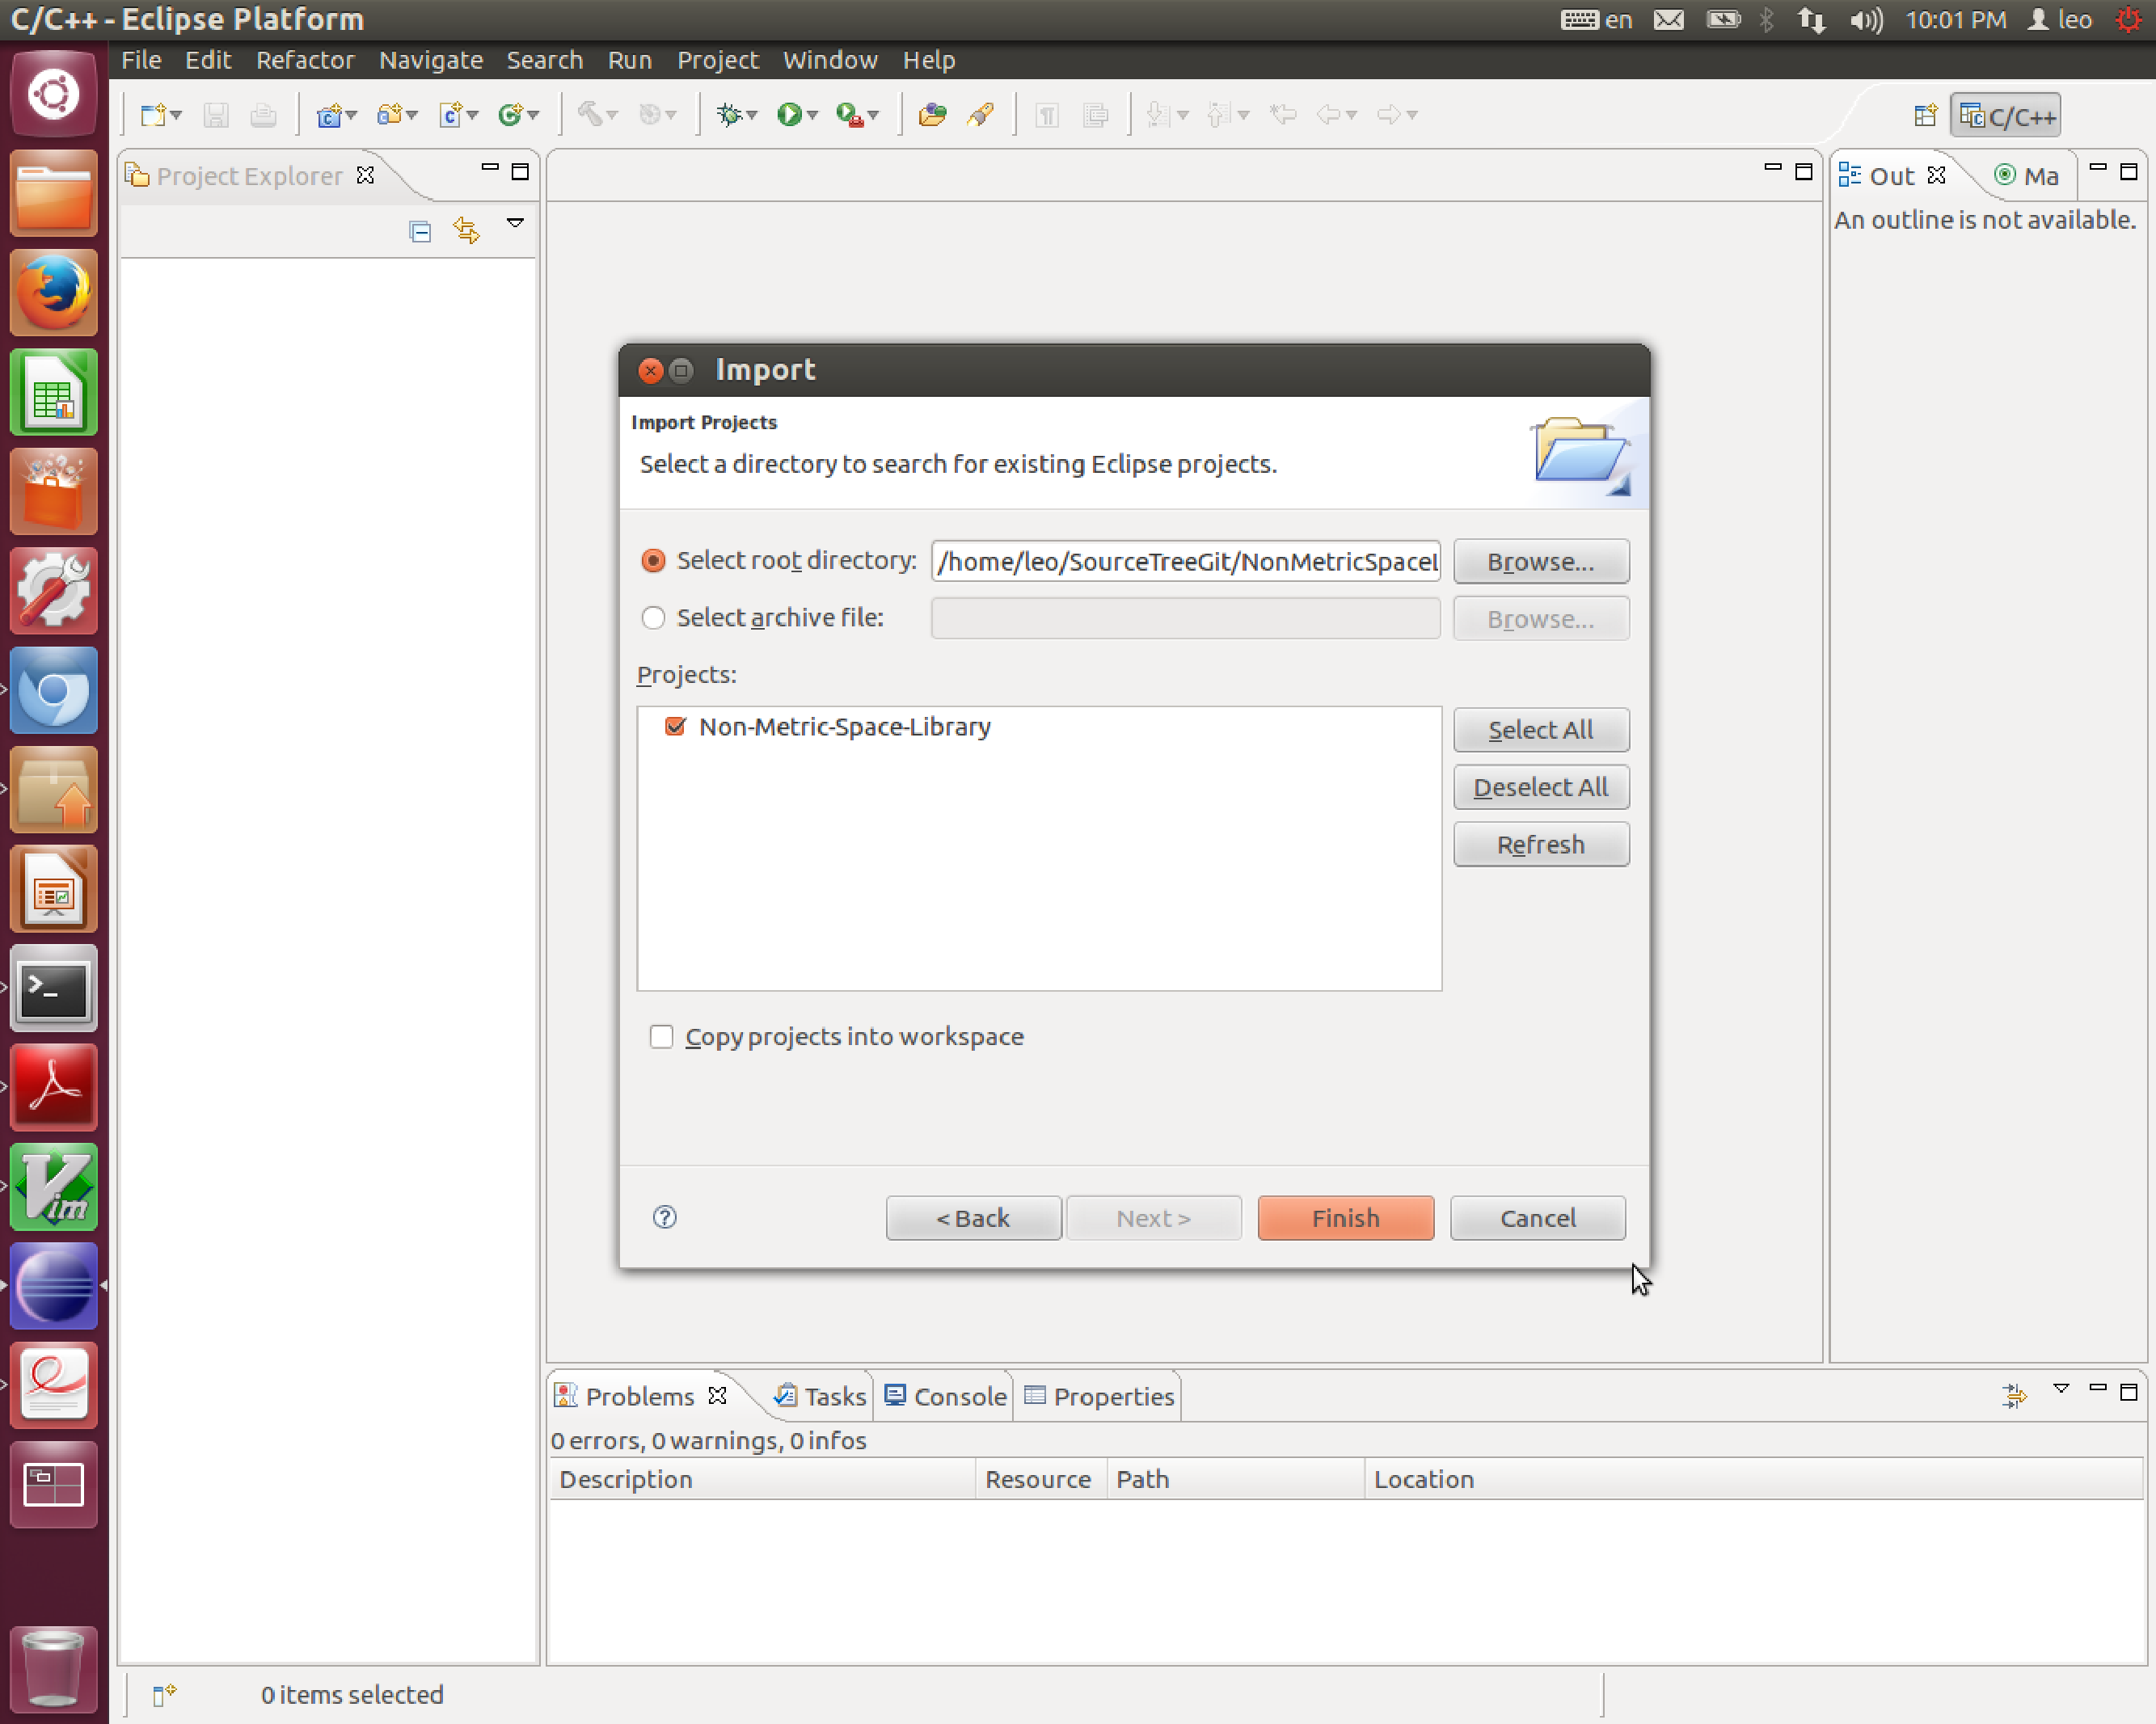
\includegraphics[width=0.9\textwidth]{figures/Eclipse2.pdf}
\end{figure}

After selecting the workspace, the user can import the Eclipse project
stored in the GitHub repository.
Go to the menu \ttt{File}, sub-menu \ttt{Import}, category \ttt{General} 
and choose to import
an existing project into the workspace as shown in Fig.~\ref{FigEclipse1}.
After that select a root directory. To this end,
go to the directory where you checked out the contents 
of the GitHub repository and enter a sub-directory \ttt{similarity\_search}.
You should now be able to see the project \ttt{Non-Metric-Space-Library}
as shown in Fig~\ref{FigEclipse2}.
You can now finalize the import by pressing the button \ttt{Finish}.

\begin{figure}
\centering
\caption{\label{FigEclipse3}Enabling indexing of the source code}
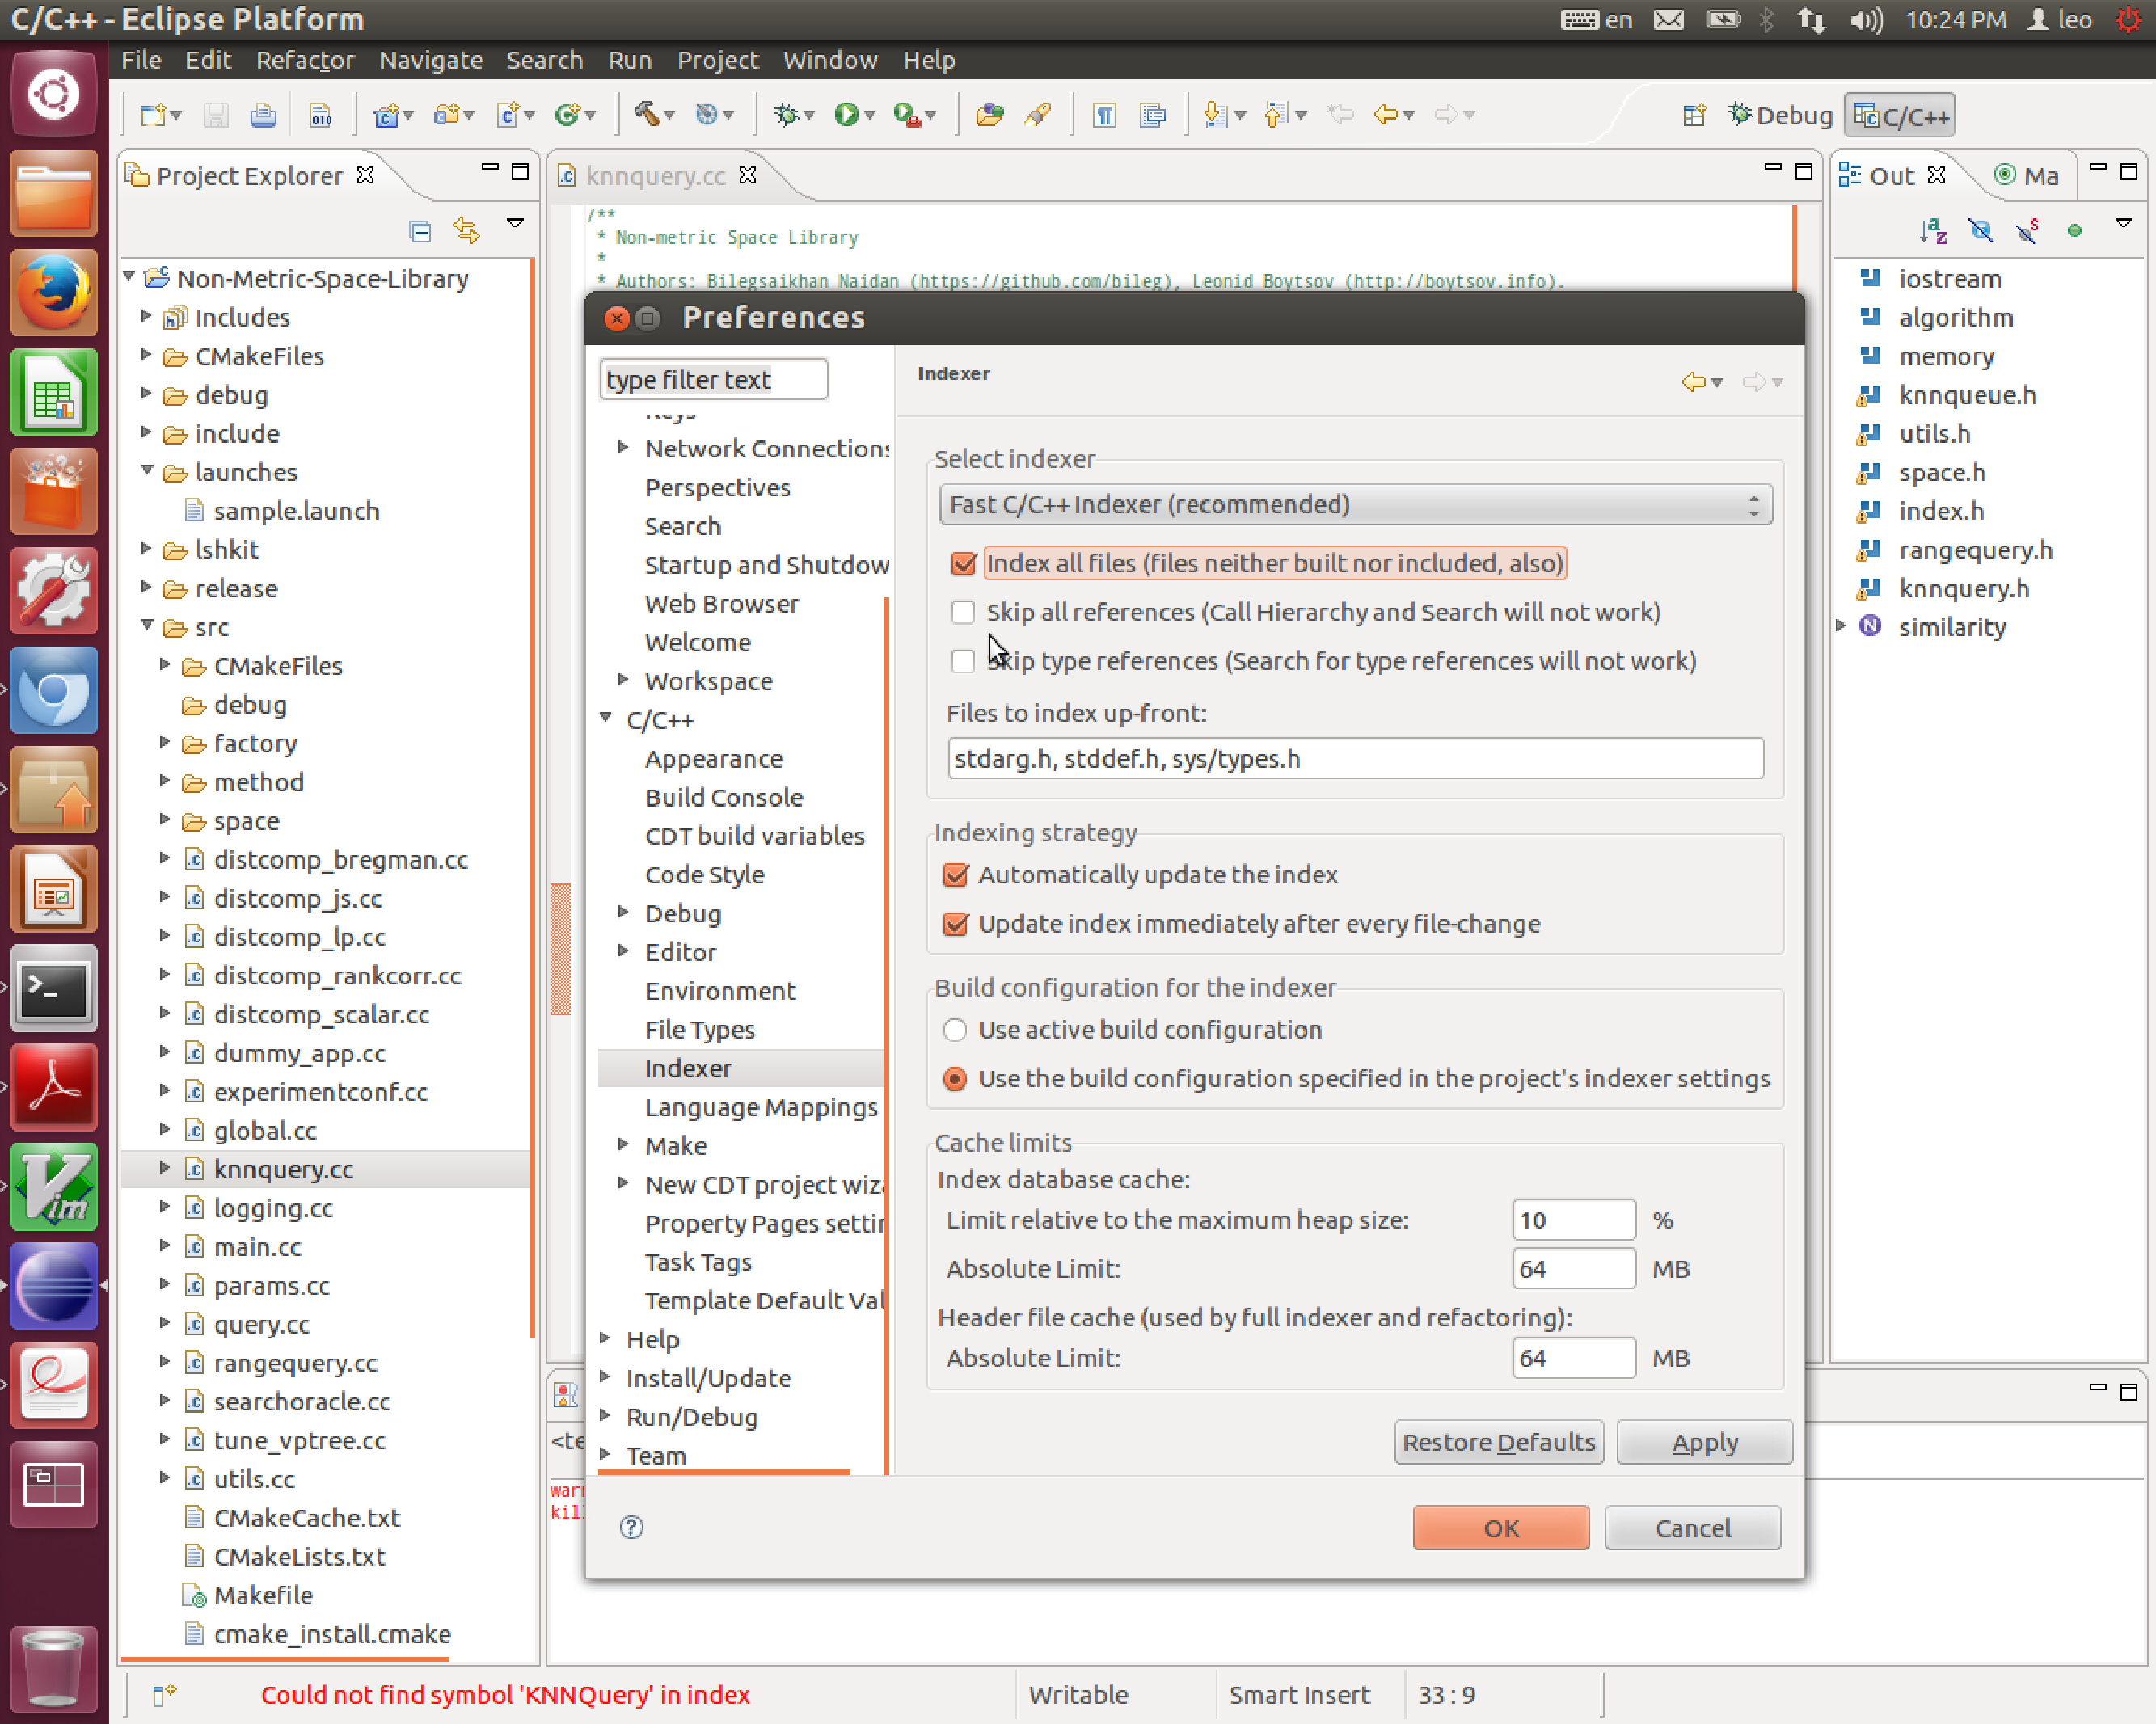
\includegraphics[width=0.9\textwidth]{figures/Eclipse3.pdf}
\end{figure}

Next, we need to set some useful settings.
Most importantly, we need to enable indexing of source files.
This would allow us to browse class hierarchies, find declarations
of variables, and classes.
To this end, go to the menu \ttt{Window}, sub-menu \ttt{Preferences}
and select a category \ttt{C++/indexing} (see Fig.~\ref{FigEclipse3}).
Then, check the box \ttt{Index all files}.
Eclipse will start indexing your files 
with the progress being shown in the status bar (right down corner).

The user can also change the editor settings. 
We would strongly encourage to disable the use of tabs.
Again, go the menu \ttt{Window}, sub-menu \ttt{Preferences}
and select a category \ttt{General/Editors/Text Editors}.
Then, check the box \ttt{Insert spaces for tabs}.
In the same menu, you can also change the fonts (use the
category \ttt{General/Appearance/Colors and Fonts}).

It is possible to build the project from Eclipse (
see the menu \ttt{Project}).
However, one first needs to generate makefiles as described in \S~\ref{SectionBuildLinux}.
The current limitation is that you can build either release
or the debug version at a time.
Moreover, to switch from one version to another, you need to recreate
the makefiles from the command line.

\begin{figure}
\centering
\caption{\label{FigDebugConf}Creating a debug/run configuration}
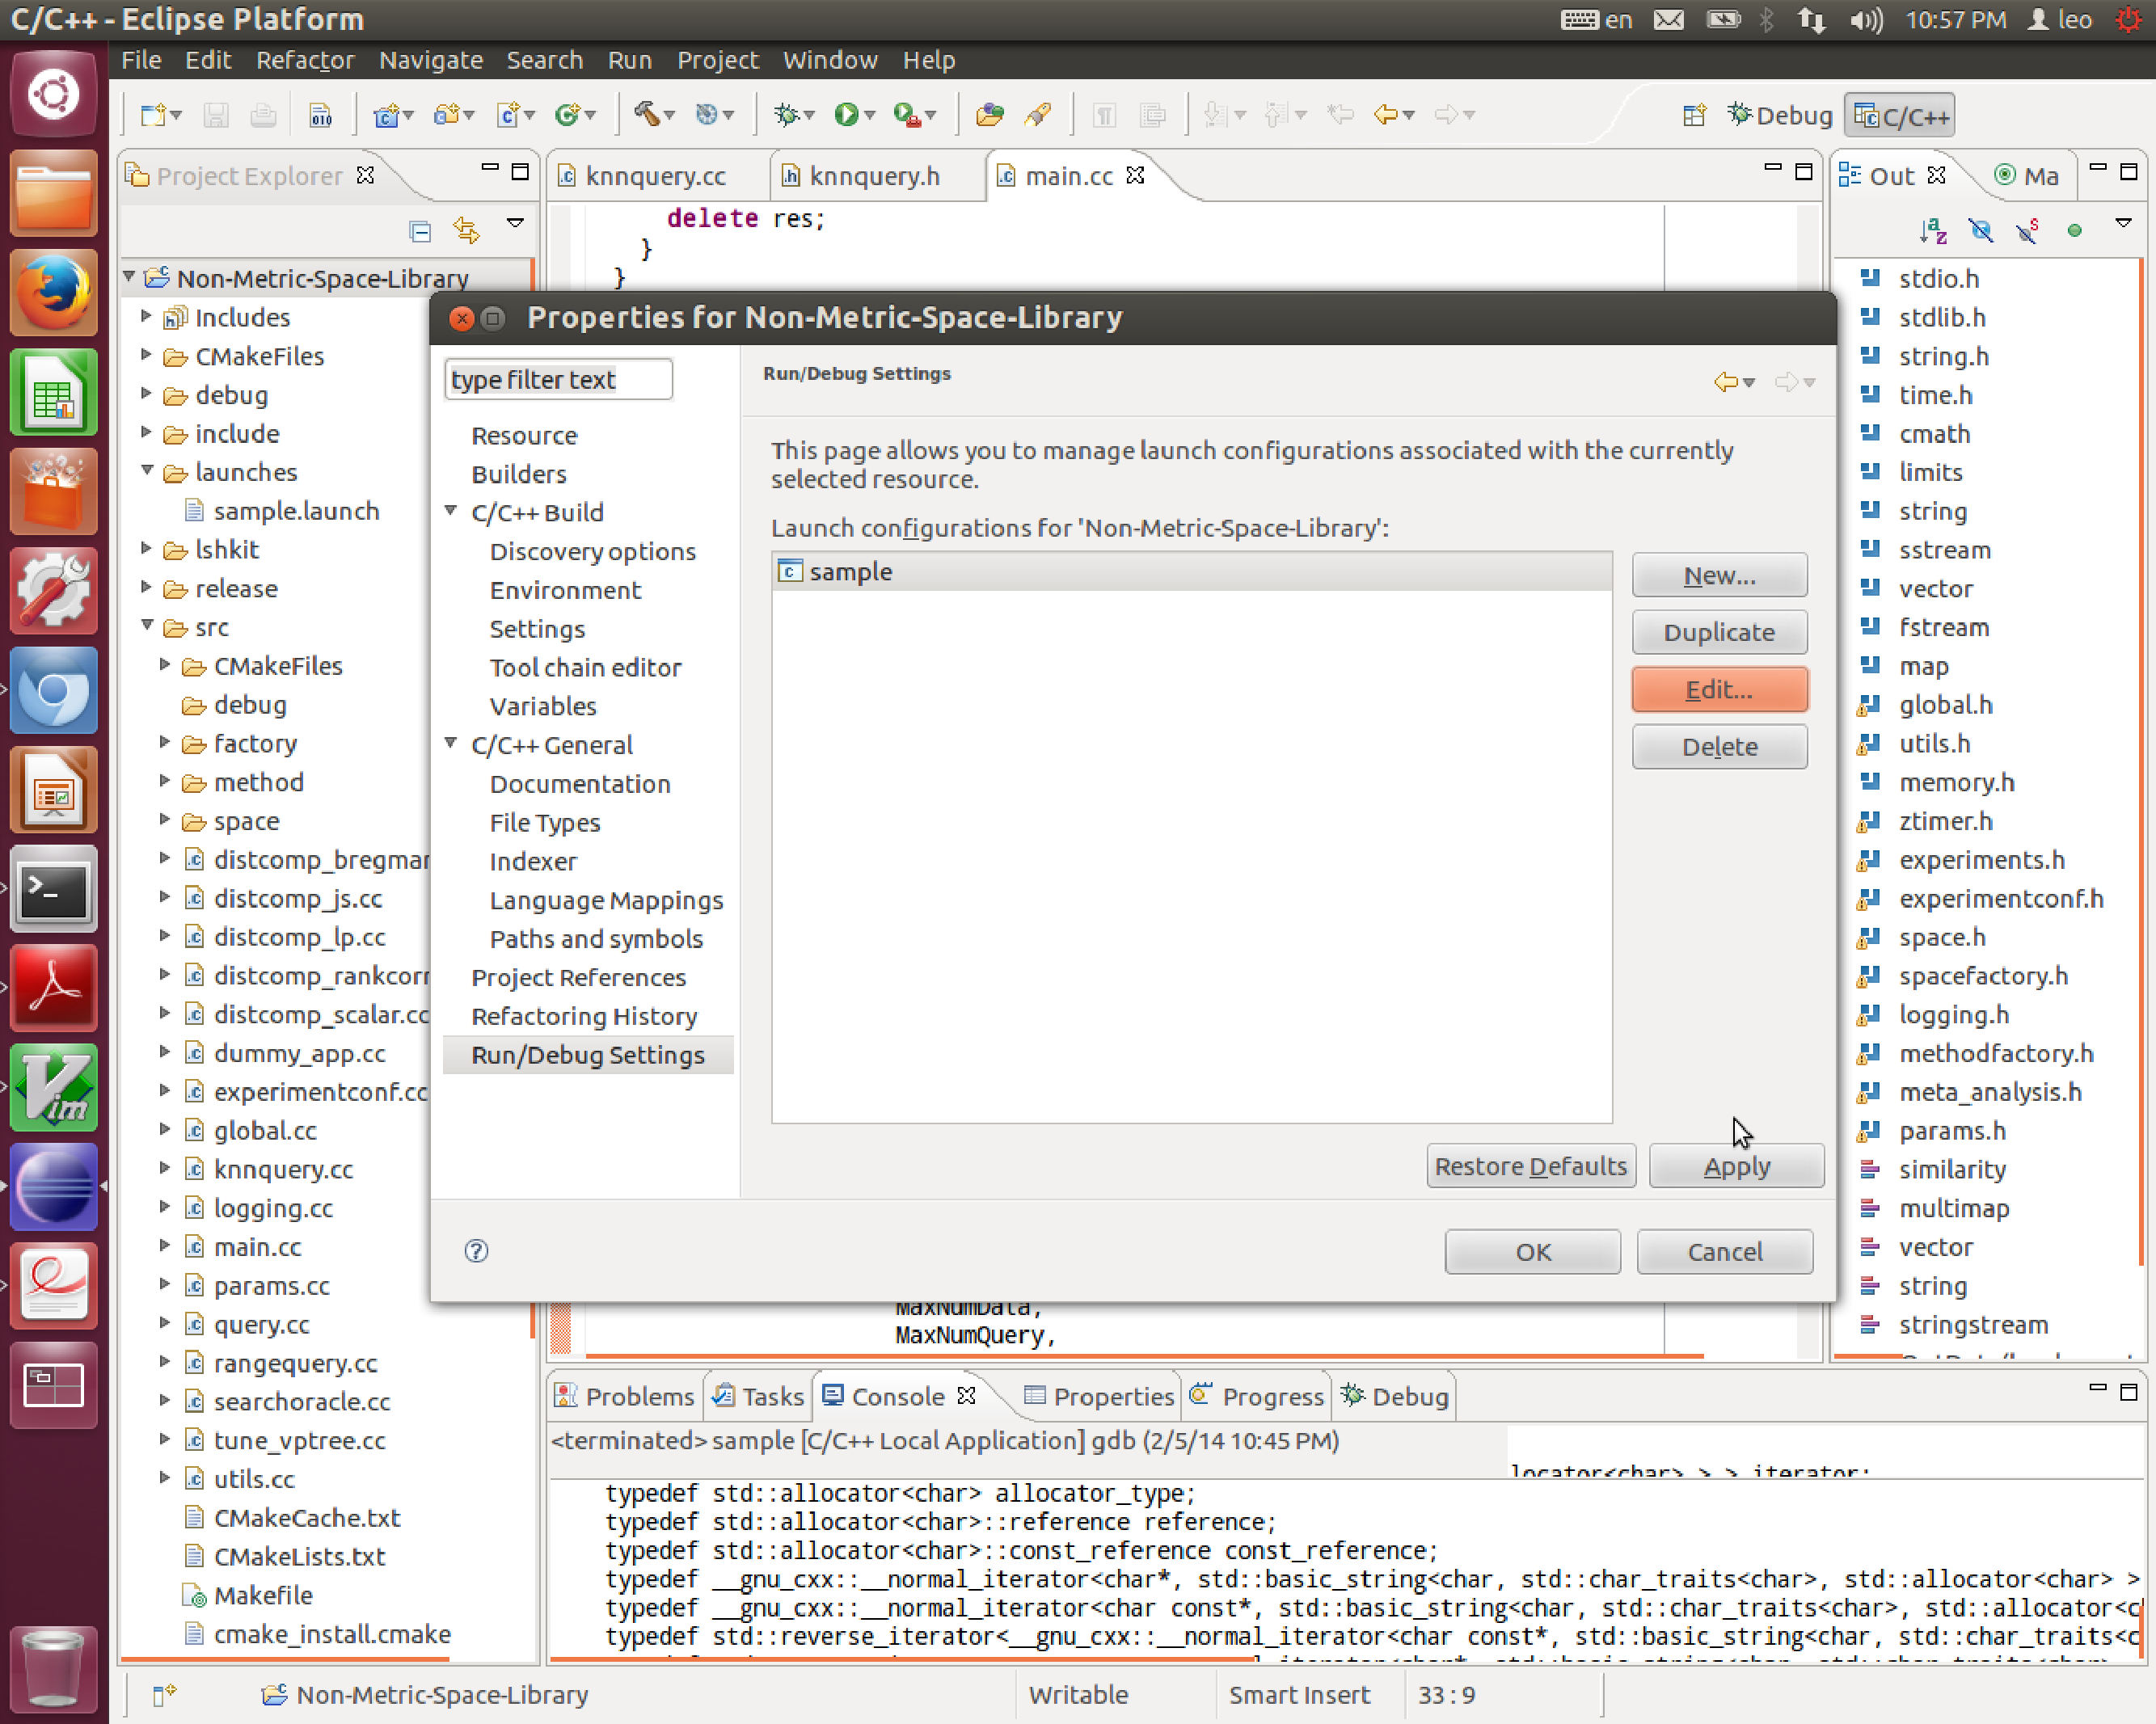
\includegraphics[width=0.9\textwidth]{figures/EclipseDebugConf.pdf}
\end{figure}

After building you can debug the project.
To do this, you need to create a debug configuration.
As an example, one configuration can be found in the 
project folder \ttt{launches}.
Right click on the item \ttt{sample.launch},
choose the option \ttt{Debug as} (in the drop-down menu),
and click on \ttt{sample} (in the pop-up menu).
After switching to a debug perspective,
the Eclipse may stop the debugger in 
the file \ttt{dl-debug.c} as shown in Fig.~\ref{FigDebug}.
If this happened, simply, press the continue icon a couple of
times until the debugger enters the code belonging to the library.

Additional configurations can be created by right clicking
on the project name (left pane), selecting \ttt{Properties}
in the pop-up menu and clicking on \ttt{Run/Debug settings}. 
The respective screenshot is shown in Fig.~\ref{FigDebugConf}.


\begin{figure}
\centering
\caption{\label{FigDebug}Starting a debugger}
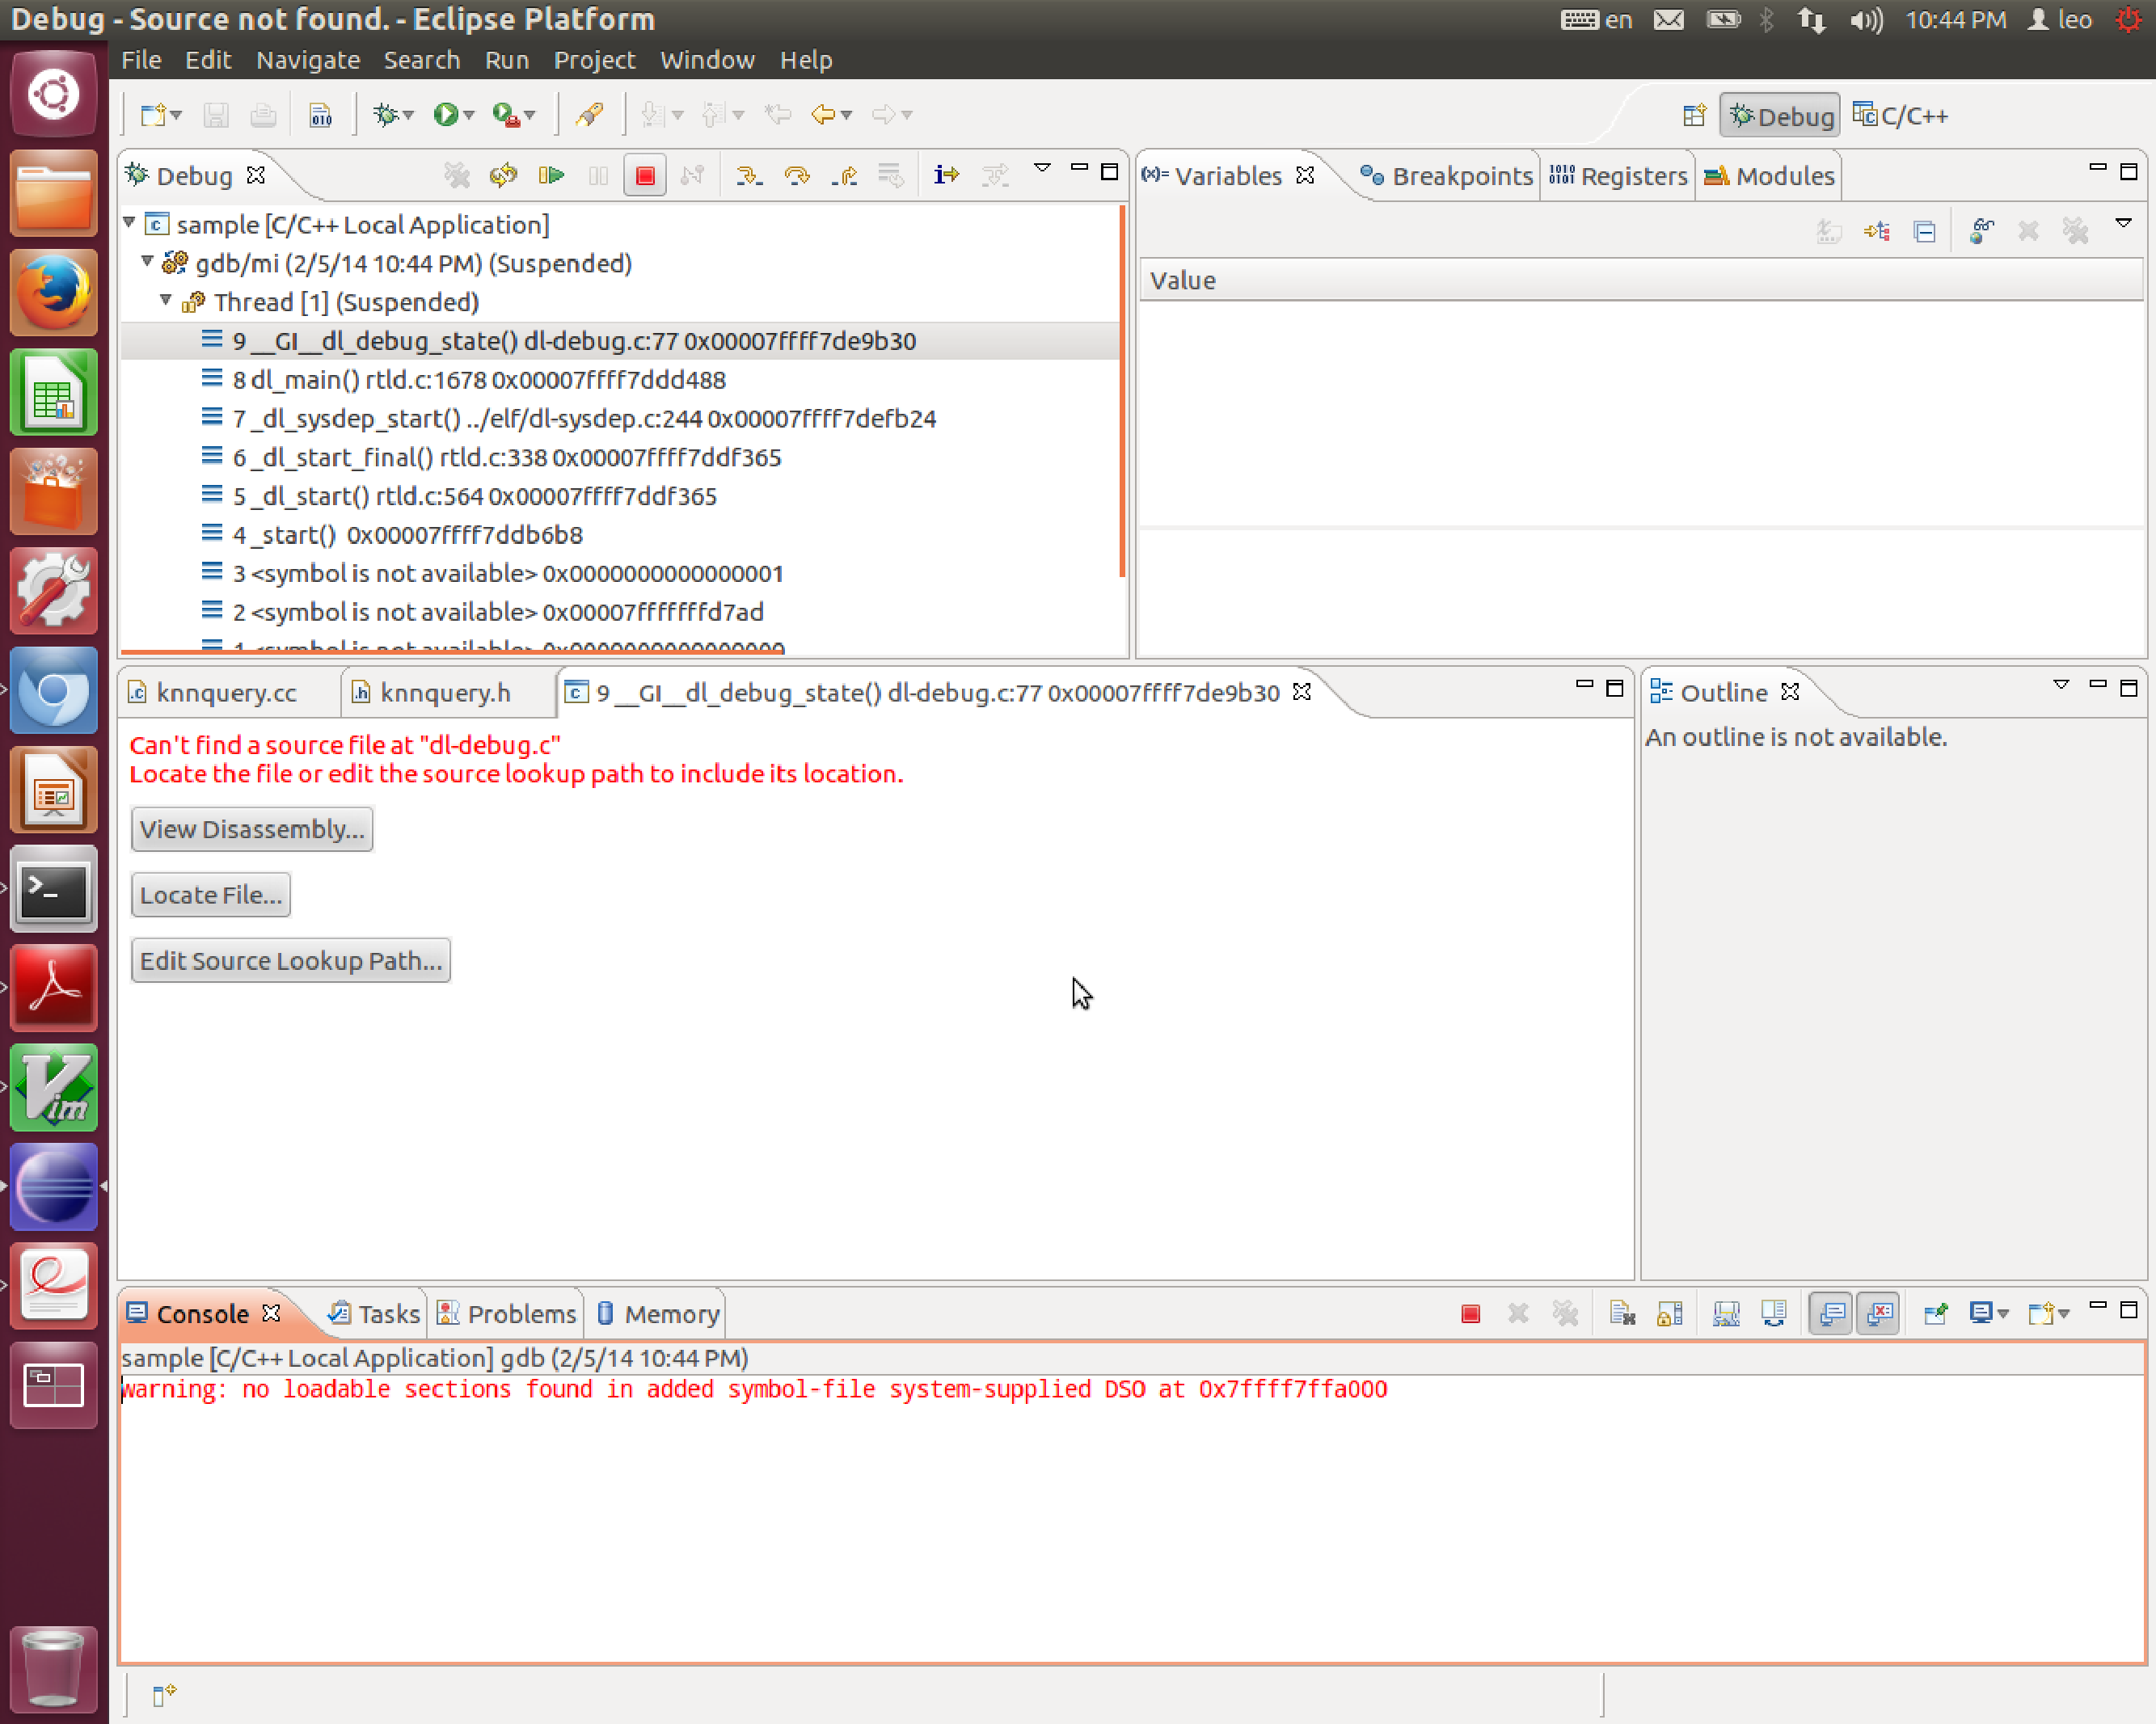
\includegraphics[width=0.9\textwidth]{figures/EclipseDebug.pdf}
\end{figure}


Note that this manual contains only a basic introduction.
If the user is new to Eclipse, we recommend reading
additional \href{http://www.eclipse.org/downloads/moreinfo/c.php}{documentation available online}.


\subsection{Building under Windows}\label{SectionBuildWindows}

\begin{figure}
\centering
\caption{\label{FigAVXSet}Specifying Location of Boost libraries}
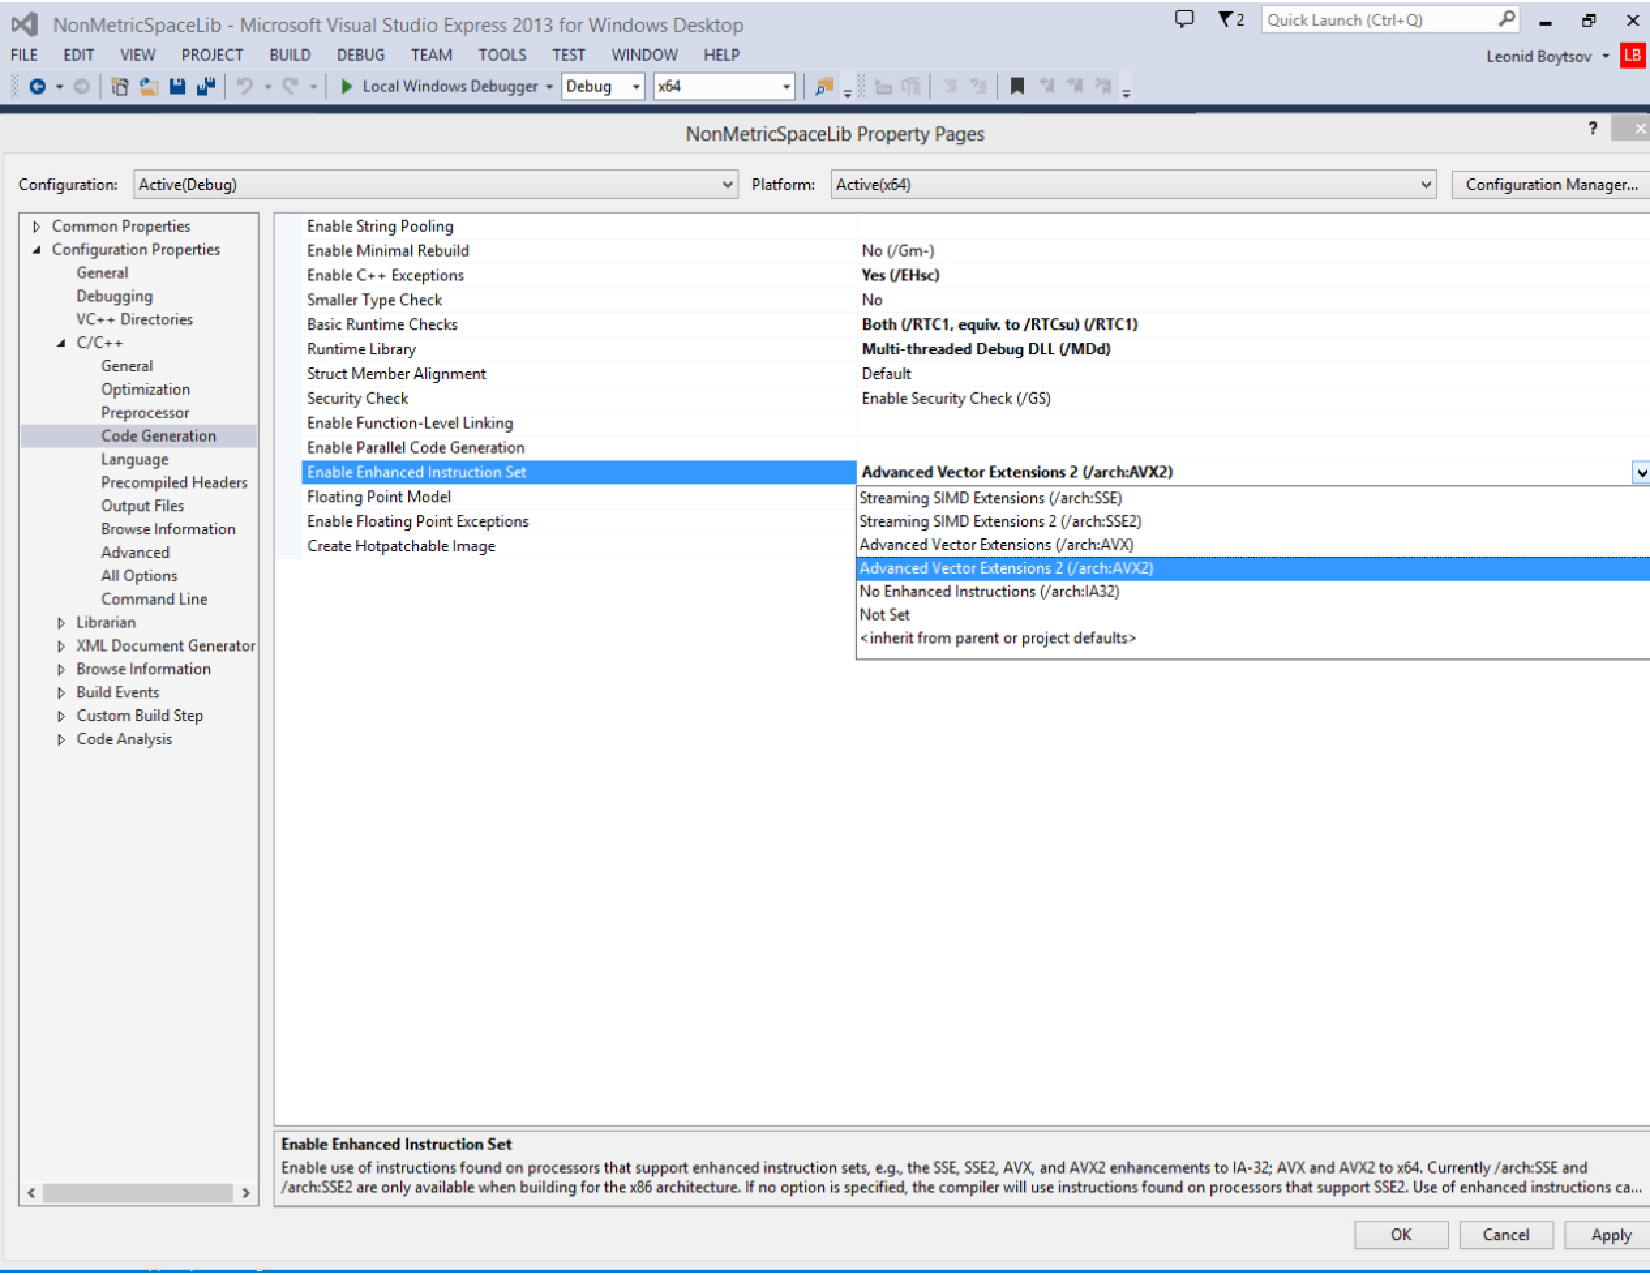
\includegraphics[width=0.9\textwidth]{figures/SettingAVXinVS2012.pdf}
\end{figure}

It is straightforward to build the project
using the provided \href{\replocfile similarity_search/NonMetricSpaceLib.sln}{Visual Studio 
solution file}.
The solution file references several (sub)-project (*.vcxproj) files,
which can be built either separately or all together.

The main sub-project is \ttt{NonMetricSpaceLib} that is built before 
any other sub-projects. 
Two sub-projects: 
\ttt{sample\_standalone\_app1},
\ttt{sample\_standalone\_app2} 
are examples of using the library in a standalone mode.
Unlike building under Linux, we provide no installation procedure yet.
In a nutshell, the installation consists in copying the library binary
as well as \href{\replocdir similarity_search/include}{the directory} with header files.

There are three possible configurations for the binaries: 
\ttt{Release}, \ttt{Debug}, and \ttt{RelWithDebInfo} (release with debug information). 
The corresponding output files are placed into the subdirectories:
\begin{verbatim}
  similarity_search\x64\Release,
  similarity_search\x64\Debug,
  similarity_search\x64\RelWithDebInfo.
\end{verbatim}

If the user's CPU supports \href{https://en.wikipedia.org/wiki/Advanced_Vector_Extensions}{AVX extensions}, it is recommended to modify code generation settings as shown in the screenshot in Fig.~\ref{FigAVXSet}.
Unlike other compilers, there seems to be no way to detect the CPU type in the Visual Studio automatically.\footnote{It is not also possible to opt for using \href{http://en.wikipedia.org/wiki/SSE4}{only SSE4}.}

\begin{figure}
\centering
\caption{\label{FigBoostSet}Specifying Location of Boost libraries}
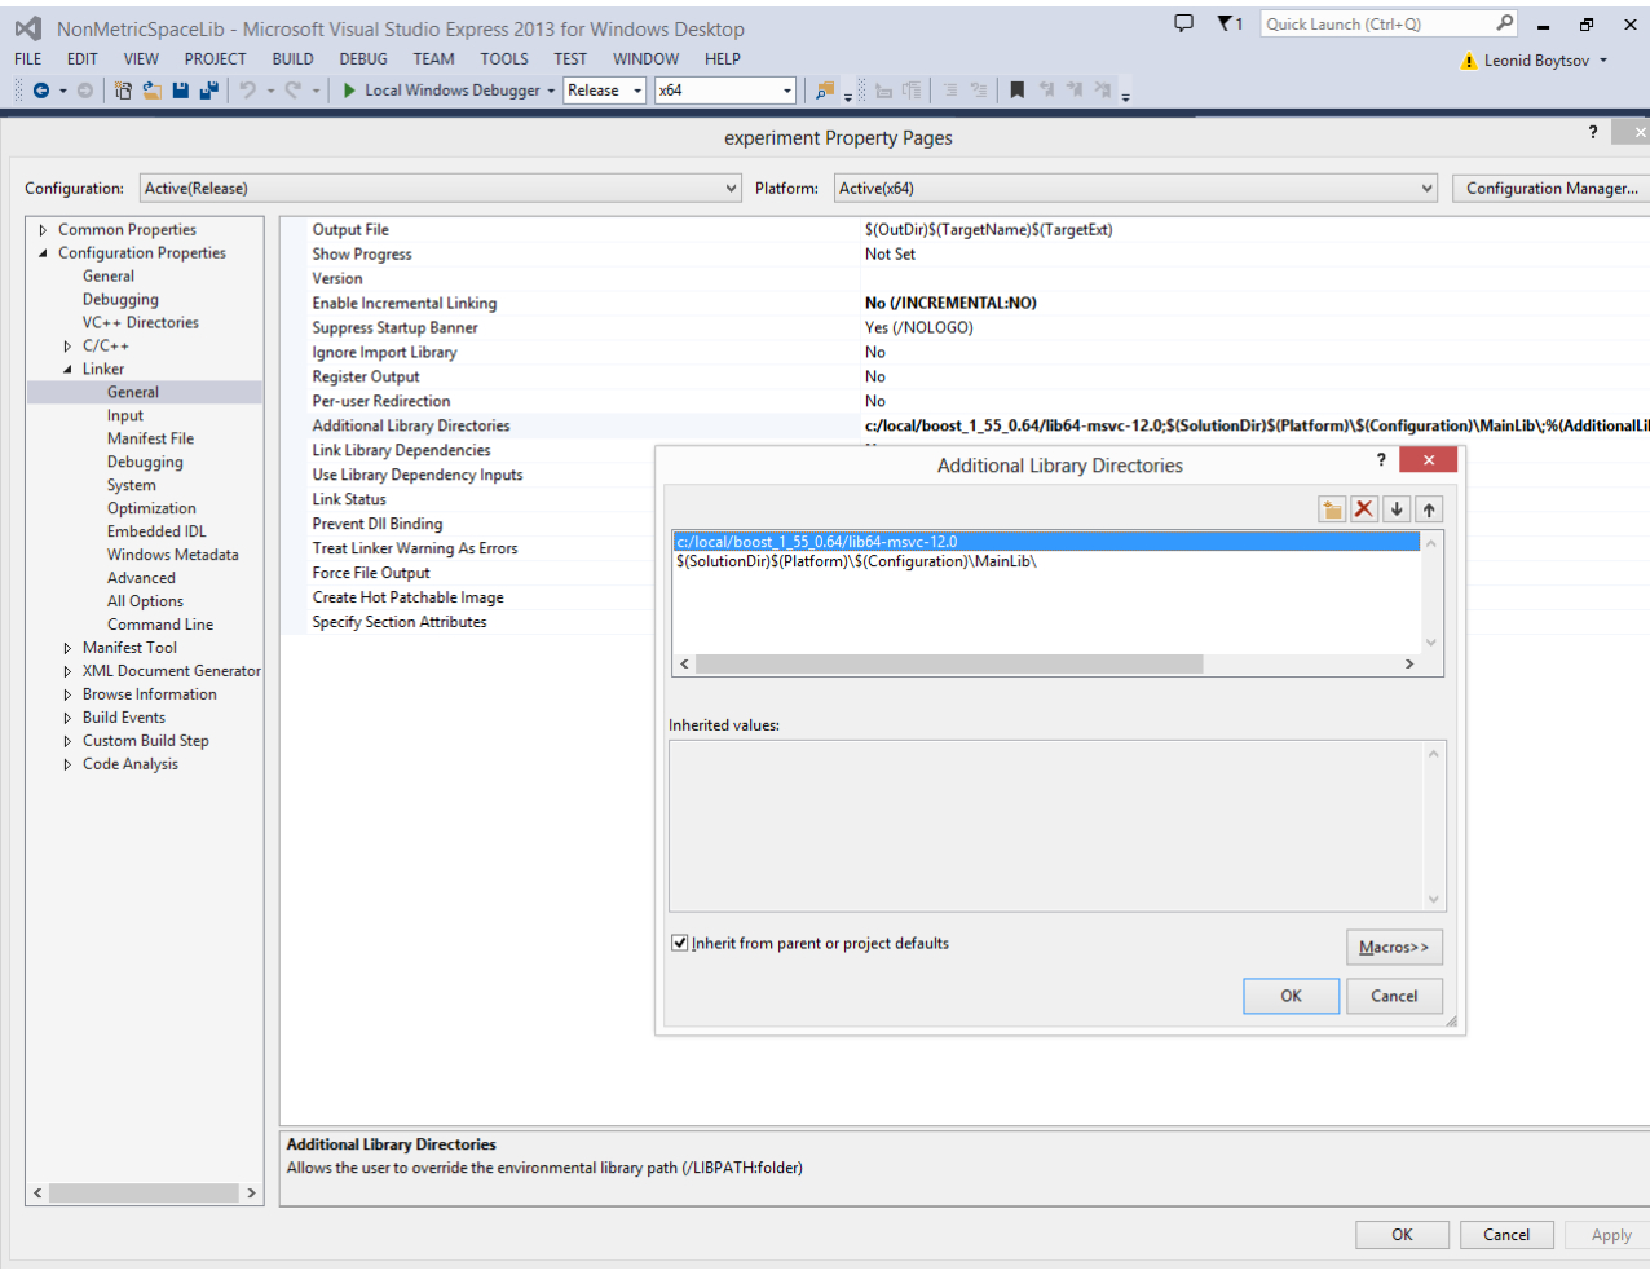
\includegraphics[width=0.9\textwidth]{figures/SettingBoostLocation.pdf}
\end{figure}

The core library, the semi unit test binary as well as examples of the standalone applications
can be built without installing Boost. 
However, Boost libraries are required for the binaries \ttt{experiment} and \ttt{tune\_vptree}.
The installer of the Boost libraries can be downloaded from \href{http://boost.teeks99.com/bin/1.55.0/}{this page}. 
Note that one needs 64-bit binaries compiled with the same version of the Visual Studio as the \nonmetrlib{} binaries.  For Visual Studio 12, one can use the following \href{http://boost.teeks99.com/bin/1.55.0/boost_1_55_0-msvc-12.0-64.exe}{download link}.

We recommend installing Boost into the folder \ttt{c:\textbackslash local\textbackslash boost\_1\_55\_0.64}. Then, no modifications of the project settings are required.
Should you install into a different folder, 
the location of Boost binaries and header file need to be specified in the 
project settings for all three build configurations (\ttt{Release}, \ttt{Debug}, \ttt{RelWithDebInfo}). An example of specifying the location of Boost libraries (binaries) is given in Fig.~\ref{FigBoostSet}.


\subsection{Running Benchmarks}\label{SectionRunBenchmark}
There are no major differences in benchmarking on Linux and Windows.
There is a one \ttt{single} benchmarking utility 
\ttt{experiment} (\ttt{experiment.exe} on Windows) that includes implementation of all methods.
It has multiple options, which specify, among others, 
a space, a data set, a type of search, and a list of methods to test (with parameters).
These options and their use cases are described in the following subsections.

\subsubsection{Space and distance value type}

A distance function can return an integer (\ttt{int}), a single-precision (\ttt{float}),
or a double-precision (\ttt{double}) real value.
A type of the distance and its value is specified as follows:

\begin{verbatim}
  -s [ --spaceType ] arg       space type, e.g., l1, l2, lp:p=0.25
  --distType arg (=float)      distance value type: 
                               int, float, double
\end{verbatim}

A description of a space may contain parameters (parameters may not contain whitespaces).
In this case, there is colon after the space mnemonic name followed by a
comma-separated (not spaces) list of parameters in the format:
\ttt{<parameter name>=<parameter value>}.
Currently, this is used only for $L_p$ spaces. For instance,
 \ttt{lp:0.5} denotes the space $L_{0.5}$.
A detailed list of possible spaces and respective
distance functions is given in Table~\ref{TableSpaces} in \S~\ref{SectionSpaces}.

For real-valued distance functions, one can use either single- or double-precision
type. Single-precision is a recommended default.\footnote{It is not clear yet,
if having double-precision distance functions is essential. Yet, we decided
to keep them. Thanks to C++ templates, it requires very little additional effort.}
We do not have a space with integer-valued distance function, but we
plan to implement an edit distance in the nearest future.

\subsubsection{Input Data/Test Set}
There are three options that define the data to be indexed:
\begin{verbatim}
  -i [ --dataFile ] arg        input data file
  --maxNumData arg (=0)        if non-zero, only the first 
                               maxNumData elements are used
  -d [ --dimension ] arg (=0)  optional dimensionality
\end{verbatim}
The input file can be indexed either completely, or partially.
In the latter case, the user can create the index using only
the first \ttt{--maxNumData} elements.
In the case of vector-space data, the dimensionality is determined
by the number of columns in the data file.
The user may choose to restrict the dimensionality and use only the first 
\ttt{--dimension} columns.

For testing, the user can use a separate test set.
It is, again, possible to limit the number of queries:
\begin{verbatim}
  -q [ --queryFile ] arg       query file
  --maxNumQuery arg (=1000)    if non-zero, use maxNumQuery query 
                               elements(required in the case 
                               of bootstrapping)
\end{verbatim}
If a separate test set is not available, it can be simulated by bootstrapping.
To this, end the \ttt{--maxNumData} elements of the original data set
are randomly divided into testing and indexable sets.
The number of queries in this case is defined by the option \ttt{--maxNumQuery}.
A number of bootstrap iterations is specified through an option:
\begin{verbatim}
  -b [ --testSetQty ] arg (=0) # of sets created by bootstrapping; 
\end{verbatim}
Benchmarking can be carried out in either a single- or a multi-threaded
mode. The number of test threads are specified as follows:
\begin{verbatim}
 --threadTestQty arg (=1)   # of threads
\end{verbatim}

\subsubsection{Query Type} 
Our framework supports the \knn and the range search.
The user can request to run both types of queries:
\begin{verbatim}
  -k [ --knn ] arg         comma-separated Ks for k-NN search
  -r [ --range ] arg       comma-separated values for range search
\end{verbatim}
For example, by specifying the options 
\begin{verbatim}
--knn 1,10 --range 0.01,0.1,1
\end{verbatim}
the user requests to run queries of five different types: $1$-NN, $10$-NN,
as well three range queries with radii 0.01, 0.1, and 1.

\subsubsection{Methods}
The following is an option to specify search methods:
\begin{verbatim}
  -m [ --method ] arg      list of method(s) with parameters
\end{verbatim}
Methods, similar to spaces, accept parameters (parameters may not contain whitespaces). 
In this case,
the name of the method is followed by a colon and a comma-separated list (no-spaces)
of parameters in the format:
\ttt{<parameter name>=<parameter value>}.
For a detailed list of methods and their parameters, please, refer to \S~\ref{SectionMethods}.

\subsubsection{Saving and Processing Benchmark Results}
The benchmarking utility outputs a detailed report (including all the log entries) to the screen
(we plan to improve logging in the nearest future).
To save benchmarking results to a file, on needs to specify a parameter:
\begin{verbatim}
  -o [ --outFilePrefix ] arg   output file prefix
\end{verbatim}
In fact, we create two files: a human-readable report (suffix \ttt{.rep}) and 
a tab-separated data file (suffix \ttt{.data}).
By default, the benchmarking utility creates files from scratch. The
following option can be used to make it work in the append mode:
\begin{verbatim}
  --appendToResFile arg (=0)   append mode flag
\end{verbatim}
For information on processing and interpreting results see \S~\ref{SectionMeasurePerf}.
A description of the plotting utility is given in \S~\ref{SectionGenPlot}.

Finally, one can redirect the output of the benchmarking utility
to a log-file:
\begin{verbatim}
  -l [ --logFile ] arg         log file
\end{verbatim}
The default behavior is to send all messages to the standard error stream.

\subsection{Measuring Performance and Interpreting Results}\label{SectionMeasurePerf}
\subsubsection{Efficiency}
Three types of efficiency indicators are used: query runtime, the number of distance computations,
and the amount of memory used by the index \emph{and} the data.
We also measure the improvement in runtime (improvement in efficiency) 
with respect to a single-thread sequential search (i.e., brute force) approach
and in the number of distance computations compared to a sequential scan method. 
For each query, this method reads compares data objects against the query.
The sequential search baseline processes \emph{all the objects}. 

The amount of memory consumed by a search method is measured indirectly: 
We record the overall memory usage of a benchmarking process before and after creation of the index. Then, we add the amount of memory used by the data.
Memory used is computed by querying special file \ttt{/dev/<process id>/status}. 
This works only for recent Linux distributives 
as we do not have a portable code to measure memory consumption of a process
(that can be used on other platforms).

\subsubsection{Effectiveness}
\label{SectionEffect}

Several effectiveness metrics are computed by the benchmarking utility:

\begin{itemize}
\item  A \emph{number of points closer} to the query than the nearest returned point.
Let $\pos(o_i)$ represent a positional distance from $o_i$ to the query, 
i.e., the number of objects closer to the query than $o_i$ plus one.
In the case of ties, we assume that the object with a smaller index is closer to the query.
Note that $\pos(o_i) \ge i$.
\item A \emph{relative position} error is equal to $\pos(o_i)/i$;
\item \emph{Recall},  which is is equal to the fraction of all correct answers retrieved.
\item \emph{Classification accuracy}, which is equal to the fraction of classed correctly
predicted by a \knn based classification procedure.
\end{itemize}

The first two metrics represent a so-called rank (approximation) error:
if we sort (i.e., rank) all the data objects with respect to their distances to the query,
where do we place objects returned by the search method?
The closer the returned objects are to the beginning of the list (i.e., 
the closer they are to to the query object), the better is the quality of the search response.

\begin{wraptable}{R}{0.52\textwidth}
\caption{An example of a human-readable report 
\label{TableHRep}}
\begin{verbatim}
===================================
vptree: triangle inequality
alphaLeft=2.0,alphaRight=2.0
===================================
# of points: 9900
# of queries: 100
------------------------------------
Recall:         0.954 -> [0.95 0.96]
ClassAccuracy:  0     -> [0 0]
RelPosError:    1.05  -> [1.05 1.06]
NumCloser:      0.11  -> [0.09 0.12]
------------------------------------
QueryTime:      0.2   -> [0.19 0.21]
DistComp:       2991  -> [2827 3155]
------------------------------------
ImprEfficiency: 2.37  -> [2.32 2.42]
ImprDistComp:   3.32  -> [3.32 3.39]
------------------------------------
Memory Usage:   5.8 MB
------------------------------------
\end{verbatim}
\textbf{Note:} \emph{confidence intervals} are in brackets
\vspace{-4em}
\end{wraptable}


Recall is a classic metric. 
It was argued, however, 
that recall does not account for position information of returned objects
and is, therefore, inferior to rank error metrics \cite{Amato_et_al:2003,Cayton:2008}.

If we specify ground-truth object classes (see \S~\ref{SectionDatasets} 
for the description of data set formats), 
it is possible to compute an accuracy of \knn based classification procedure.
The class of the element is predicted to be most frequent class label among $k$ closest objects
returned by the method (in the case of ties the class label with the smallest id is chosen).

If we had ground-truth queries and relevance judgements from human assessors (e.g.,
if a vector represents an image, it is similar to the query image?),
we could in principle compute other realistic effectiveness metrics 
such as the mean average precision,
or the normalized discounted cumulative gain.
This remains for the future work.

\subsection{Interpreting and Processing Benchmark Results}
If the user specifies the option \ttt{--outFilePrefix},
the benchmarking results are stored to the file system.
A prefix of result files is defined by the parameter \ttt{--outFilePrefix}
while the suffix is defined by a type of the search procedure (\knn or range)
as well as by search parameters (e.g., the range search radius).
For each type of search two files are generated:
a report in a human-readable format,
and a tab-separated data file intended for automatic processing.
The data file contains only the average values,
which can be used to, e.g., produce efficiency-effectiveness plots
as described in \S~\ref{SectionGenPlot}.

%\todonoteinline{Gotchas with specifying the query-time parameters}

An example of human readable report (\emph{confidence intervals} are in square brackets)
is given in Table~\ref{TableHRep}.
In addition to averages, the human-readable report provides 95\% confidence intervals.
In the case of bootstrapping, statistics collected for several splits of the data set are aggregated.
For the retrieval time and the number of distance computations,
this is done via a classic fixed-effect model adopted in meta analysis \cite{Hedges_and_Vevea:1998}.
When dealing with other performance metrics, 
we employ a simplistic approach of averaging split-specific values
and computing the sample variance over spit-specific averages.\footnote{The distribution
of many metric values was not normal. There are approaches to resolve this issue (e.g., apply a transformation),
but an additional investigation is needed to understand which approaches work best.}
Note for all metrics, except relative position error, an average is computed using an arithmetic mean.
For the relative error, however, we use the geometric mean  \cite{king:1986}.


\subsection{Plotting results}\label{SectionGenPlot}
We provide the Python script to generate performance graphs 
from tab-separated data file produced by the 
benchmarking utility \ttt{experiment}. 
The plotting script is \href{\replocfile sample_scripts/sample_scripts/genplot.py}{genplot.py} (see \S~\ref{SectionGenPlot}).
In addition to Python, this script requires Latex and PGF. 

Consider the following example of using \ttt{genplot.py}:
\begin{verbatim}
../sample_scripts/genplot.py  \
           -i result_K\=1.dat -o plot_1nn \
           -x 1~norm~Recall \
           -y 1~log~ImprEfficiency \
           -l "2~(0.96,-.2)" \
           -t "ImprEfficiency  vs Recall"
\end{verbatim}

It aims to process the output tab-separated data file \ttt{result\_K=1.dat},
which was generated for 1-NN search, and save the plot to the file \ttt{plot\_1nn.pdf}.
Note that one should not explicitly specify the extension of the output file (as
\ttt{.pdf} is always implied).

Parameters \ttt{-x} and \ttt{-y} define  X and Y axis and have the same format.
Each parameter has three tilda-separated entities. The first should
be 0 or 1. Specify 0, only if do not want to print the axis label.
The second entitity is either \ttt{norm} or \ttt{log}, 
which stands for a normal or logarithmic scale, respectively.
The last entity defines a metric that we want to visualize:
It should one of the names that appear in the first row of the output data file.
The title of the plot is defind by \ttt{-t}.
The parameter \ttt{-l} defines a plot legend.
It is either a string \ttt{none} (to hide the legend) 
or  it contains two tilda-separated entities.

The first entity gives the number of columns in the legend, while the second entity
defines a position of the legend. The position can be either an explicity
point (in round brackets) or one of the following descriptors of the
relative position (quotes are for clarity only): ``north west'', ``north east'', ``south west'', ``south east''.
If the relative position is specified, the legend is printed insided the main
plotting area, e.g.:
\begin{verbatim}
../sample_scripts/genplot.py  \
           -i result_K\=1.dat -o plot_1nn \
           -x 1~norm~Recall \
           -y 1~log~ImprEfficiency \
           -l "2~north west" \
           -t "ImprEfficiency  vs Recall"
\end{verbatim}


\section{Spaces}\label{SectionSpaces}
Currently we provide implementations only for vector spaces,
but this is not a principal limitation.
The input files can come in either regular, i.e., dense,
or sparse variant (see \S~\ref{SectionDatasets}). 

For a detailed list of spaces, their parameters, 
and performance characteristics is given in Table~\ref{TableSpaces}.
The mnemonic name of the space is passed to the benchmarking utility (see \S~\ref{SectionRunBenchmark}).
There can be more than one version of a distance function,
which have different space-performance trade-off.
In particular, for distances that require computation of logarithms 
we can achieve an order of magnitude improvement (for the GNU C++) by precomputing
logarithms at index time. This comes at a price of extra storage. 
In the case of Jensen-Shannon distance functions, we can pre-compute some 
of the logarithms and accurately approximate those we cannot pre-compute.
The details are explained in \S~\ref{SectionLP}-\ref{SectionBregman}.

Straightforward slow implementations of the distance functions may have the substring \ttt{slow}
in their names, while faster versions contain the substring \ttt{fast}.
Fast functions that involve approximate computations contain additionally the substring \ttt{approx}.
For non-symmetric distance function, a space may have two variants: one variant is for left
queries (the query object is the first argument of the distance function) 
and another is for right queries (the query object is the second argument).
In the latter case the name of the space ends on \ttt{rq}.
Separating spaces by query types, might not be the best approach.
Yet, it seems to be unavoidable, because, in many cases,
we need separate indices for left and right queries.

Distance computation efficiency was evaluated on a Core i7 laptop (3.4 Ghz peak frequency)
in a single-threaded mode (by the utility \href{\replocfile similarity_search/test/bunit.cc}{bunit}).
It is measured in millions of computations per second for single-precision
floating pointer numbers (double precision computations are, of course, more costly). 
The code was computed using the GNU compiler. 
Somewhat higher efficiency numbers can be obtained by using the Intel compiler.
In fact, performance is much better for distances relying on ``heavy'' math functions:
slow versions of KL- and Jensen-Shannon divergences and Jensen-Shannon metrics, 
as well as for $L_p$ spaces,
where $p \not\in\{1,2,\infty\}$.

In the efficiency test, all dense vectors have 128 elements.
For all dense-vector distances except the Jensen-Shannon divergence,
their elements were generated randomly and uniformly.
For the Jensen-Shannon divergence, we first generate elements randomly,
and next we randomly select elements that are set to zero (approximately half). 
Additionally, for KL-divergences and the JS-divergence,
we normalize vector elements so that they correspond a true discrete probability distribution. 
Sparse space distances were tested using sparse vectors from a small sample file in the
\href{\replocfile sample_data/sparse_5K.txt}{sample\_data} directory.

\hspace{-2em}\begin{table}
\caption{Description of implemented spaces\label{TableSpaces}}
\centering
\begin{tabular}{l@{\hspace{2mm}}l@{\hspace{2mm}}l}
\toprule
\textbf{Space}& \textbf{Mnemonic Name \& Formula}   & \textbf{Efficiency} \\
              &                           & (million op/sec) \\
\toprule
\multicolumn{3}{c}{\textbf{Metric Spaces}}  \\
\toprule
Hamming &  \ttt{bit\_hamming}                      &  240 \\
                 &  $\sum_{i=1}^n |x_i-y_i|$                         &  \\
\cmidrule(l){1-3} 
$L_1$     &  \ttt{l1}, \ttt{l1\_sparse}              &                   35, 1.6 \\
                 &  $\sum_{i=1}^n |x_i-y_i|$                         &  \\
\cmidrule(l){1-3} 
$L_2$     &  \ttt{l2}, \ttt{l2\_sparse}              &                  30, 1.6  \\
                 & $\sqrt{\sum_{i=1}^n |x_i-y_i|^2}$                 &   \\
\cmidrule(l){1-3} 
$L_{\infty}$ &  \ttt{linf}, \ttt{linf\_sparse}      &   34 , 1.6  \\
                    & $\max_{i=1}^n |x_i-y_i|$           & \\
\cmidrule(l){1-3} 
$L_p$ (generic $p \ge 1$)& \ttt{lp:p=\ldots}, \ttt{lp\_sparse:p=\ldots}  &  0.1-3, 0.1-1.2  \\
                                & $\left(\sum_{i=1}^n |x_i-y_i|^p\right)^{1/p}$  & \\
\cmidrule(l){1-3} 
Angular distance & \ttt{angulardist}, \ttt{angulardist\_sparse}, \ttt{angulardist\_sparse\_fast} & { 13, 1.4, 3.5 } \\
                        & $\arccos\left(1-\frac{\sum_{i=1}^n x_i y_i}{\sqrt{\sum_{i=1}^n x_i^2}\sqrt{\sum_{i=1}^n y_i^2 }}\right)$   & \\
\cmidrule(l){1-3} 
Jensen-Shan. metr. &\ttt{jsmetrslow, jsmetrfast, jsmetrfastapprox} &  0.3, 1.9, 4.8  \\
                          & $\sqrt{\frac{1}{2}\sum_{i=1}^n \left[x_i \log x_i + y_i \log y_i  - (x_i+y_i)\log \frac{x_i +y_i}{2}\right]}$  & \vspace{1em} \\
\toprule
\multicolumn{3}{c}{\textbf{Non-metric spaces (symmetric distance)}}  \\
\toprule
$L_p$ (generic $p < 1$)& \ttt{lp:p=\ldots, lp\_sparse:p=\ldots}                     &  0.1-3, 0.1-1 \\
                              & $\left(\sum_{i=1}^n |x_i-y_i|^p\right)^{1/p}$  &   \\
\cmidrule(l){1-3} 
Jensen-Shan. div. &\ttt{jsdivslow, jsdivfast, jsdivfastapprox} &   0.3, 1.9, 4.8 \\
                          & $\frac{1}{2}\sum_{i=1}^n \left[x_i \log x_i + y_i \log y_i  - (x_i+y_i)\log \frac{x_i +y_i}{2}\right]$ & \\
\cmidrule(l){1-3} 
Cosine similarity & \ttt{cosinesimil}, \ttt{cosinesimil\_sparse}, \ttt{cosinesimil\_sparse\_fast} & { 13, 1.4, 3.5 } \\
                        & $1-\frac{\sum_{i=1}^n x_i y_i}{\sqrt{\sum_{i=1}^n x_i^2}\sqrt{\sum_{i=1}^n y_i^2 }}$   & \vspace{1em} \\
\toprule
\multicolumn{3}{c}{\textbf{Non-metric spaces (non-symmetric distance)}}  \\
\toprule
regular KL-div. & left queries: \ttt{kldivfast}       & 0.5, 27 \\
                       & right queries: \ttt{kldivfastrq}    &  \\
                       & $\sum_{i=1}^n   x_i \log \frac{x_i}{y_i}$  & \\ 
\cmidrule(l){1-3} 
generalized KL-div. & left queries: \ttt{kldivgenslow}, \ttt{kldivgenfast} & 0.5, 27    \\
                           & right queries: \ttt{kldivgenfastrq} & 27    \\
                           & $\sum_{i=1}^n \left[  x_i \log \frac{x_i}{y_i} -   x_i +   y_i \right]$   &   \\
\cmidrule(l){1-3} 
Itakura-Saito & left queries: \ttt{itakurasaitoslow, itakurasaitofast}   & 0.2, 3, 14 \\
              & right queries: \ttt{itakurasaitofastrq}                  & 14         \\
              & $\sum_{i=1}^n \left[ \frac{ x_i}{y_i} - \log \frac{x_i}{y_i}  -1 \right]$ \\
\toprule
\end{tabular}
\end{table}

\subsection{$L_p$-norms}\label{SectionLP}
The $L_p$ distance between vectors $x$ and $y$ are
given by the formula:
\begin{equation}\label{EqMink}
L_p(x,y) = \left(\sum_{i=1}^n |x_i-y_i|^p\right)^{1/p}
\end{equation}
In the limit ($p \rightarrow \infty$),
the $L_p$ distance becomes the Maximum metric, also known as 
the Chebyshev distance:
\begin{equation}\label{EqCheb}
L_{\infty}(x,y) = \max\limits_{i=1}^n |x_i-y_i|
\end{equation}
$L_{\infty}$ and all spaces $L_p$ for $p \ge 1$
are true metrics. 
They are symmetric, equal to zero only for identical elements,
and, most importantly, satisfy \emph{the triangle inequality}.
However, the $L_p$ norm is \emph{not} a metric if $p<1$.

In the case of dense vectors, 
we have reasonably efficient implementations 
for $L_p$ distances where $p$ is either integer or infinity. 
The most efficient implementations are for $L_1$ (Manhattan),
$L_2$ (Euclidean), and $L_{\infty}$ (Chebyshev).
As explained in Leo's blog,
\href{http://searchivarius.org/blog/efficient-exponentiation-square-rooting}{we compute exponents through square rooting}. 
This works best when the number of digits (after the binary digit) is small, e.g., if $p=0.125$.

Any $L_p$ space can have a dense and a sparse variant.
Sparse vector spaces have their own mnemonic names, which are different
from dense-space mnemonic names in that they contain a suffix \ttt{\_sparse} (see also Table~\ref{TableSpaces}).
For instance \ttt{l1} and \ttt{l1\_sparse} are both $L_1$ spaces,
but the former is dense and the latter is sparse.
The mnemonic names of $L_1$, $L_2$, and $L_\infty$ spaces (passed to the benchmarking utility) are
\ttt{l1}, \ttt{l2}, and \ttt{linf}, respectively.
Other generic $L_p$ have the name $lp$, which is used in combination with a parameter.
For instance, $L_3$ is denoted as \ttt{lp:p=3}.

Distance functions for sparse-vector spaces are far less efficient, 
due to a costly, branch-heavy, operation of matching sparse vector indices
(between two sparse vectors).

\subsection{Scalar-product Related Distances}
We have two distance function whose formulas include normalized scalar product.
One is the cosine similarity, which is equal to:
$$
d(x,y) =1-\frac{\sum_{i=1}^n x_i y_i} 
{\sqrt{\sum_{i=1}^n x_i^2} \sqrt{\sum_{i=1}^n y_i^2 } } 
$$ 
The cosine similarity is not a true metric, but it can be converted into
one by applying a monotonic transformation (i.e.., taking an inverse cosine).
The resulting distance function is a true metric that 
is called the angular distance.
The angular distance is computed using the following formula:
$$
d(x,y) =\arccos\left(1-\frac{\sum_{i=1}^n x_i y_i} 
{\sqrt{\sum_{i=1}^n x_i^2} \sqrt{\sum_{i=1}^n y_i^2 } }\right) 
$$ 

In the case of sparse spaces, to compute the scalar product,
we need to obtain an intersection of vector element ids
corresponding to non-zero elements.
A classic text-book intersection algorithm (akin to a merge-sort)
is not particularly efficient, apparently,
due to frequent branching.
For \emph{single-precision} floating point vector elements,
we provide a more efficient implementation that relies on the 
all-against-all comparison SIMD instruction \texttt{\_mm\_cmpistrm}.
This implementation  (inspired by the set intersection algorithm of Schlegel~et~al.~\cite{schlegel2011fast})
is about 2.5 times faster than a pure C++ implementation based on the merge-sort approach.

\subsubsection{Jensen-Shannon divergence}\label{SectionJS}
\emph{Jensen-Shannon} divergence is a symmetrized and smoothed KL-divergence:
\begin{equation}\label{EqJS}
\frac{1}{2}\sum_{i=1}^n\left[ x_i \log x_i + y_i \log y_i  -(x_i+y_i)\log \frac{x_i +y_i}{2}\right]
\end{equation}
This divergence is symmetric, but it is not a metric function.
However, the square root of the Jensen-Shannon divergence
is a proper a metric \cite{endres2003new},
which we call the Jensen-Shannon metric.

A straightforward implementation of Eq.~\ref{EqJS} is inefficient for two reasons 
(at least when one uses the GNU C++ compiler)
(1) computation of logarithms is a slow operation (2)
the case of zero $x_i$ and/or $y_i$ requires conditional processing, i.e.,
costly branches.

A better method is to pre-compute logarithms of data at index time. 
It is also necessary to compute logarithms of a query vector.
However, this operation has a little cost since it is carried out once 
for each nearest neighbor or range query.
Pre-computation leads to a 3-10 fold improvement depending on the sparsity of vectors,
albeit at the expense of requiring twice as much space.
Unfortunately, it is not possible to avoid computation of the third logarithm:
it needs to be computed in points that are not known until we see the query vector.

However, it is possible to approximate it with a very good precision,
which should be sufficient for the purpose of approximate searching.
To this end, we rewrite Equation \ref{EqJS} as follows:
$$
\frac{1}{2}\sum_{i=1}^n\left[ x_i \log x_i + y_i \log y_i  -(x_i+y_i)\log \frac{x_i +y_i}{2}\right]=
$$
$$
 = \frac{1}{2}\sum_{i=1}^n\left[ x_i \log x_i + y_i \log y_i\right]  -
\sum_{i=1}^n\left[\frac{(x_i+y_i)}{2}\log \frac{x_i +y_i}{2} \right]=
$$
$$
 = \frac{1}{2}\sum_{i=1}^n x_i \log x_i + y_i \log y_i  -
$$
\begin{equation}\label{Eq1}
\sum_{i=1}^n\frac{(x_i+y_i)}{2}\left[\log\frac{1}{2} + \log \max(x_i,y_i) + 
\log \left(1 + \frac{\min(x_i,y_i)}{\max(x_i,y_i)}\right) \right]
\end{equation}
We can pre-compute all the logarithms in Eq.~\ref{Eq1} except for $\log \left(1 + \frac{\min(x_i,y_i)}{\max(x_i,y_i)}\right) $. However, its argument value is in a small range: from one to two.
We can discretize the range, compute logarithms in many intermediate points and save the computed values in a table.
Finally, we employ the SIMD instructions to implement this approach. 
As our tests show, this is a very efficient approach, which results in a very little (around $10^{-6}$ on average) relative error for the value of the Jensen-Shannon divergence.

Another possible approach is use \href{http://fastapprox.googlecode.com/svn/trunk/fastapprox/src/fastonebigheader.h}{an efficient approximation for logarithm computation}.
However, \href{https://github.com/searchivarius/BlogCode/tree/master/2013/12/26}{as our tests show},
this method is still relatively slow (it takes almost 20 CPU cycles per log),
 while the relative error is as high as $3 \cdot 10^{-4}$ for logarithm arguments smaller than 2.

\subsection{Bregman Divergences}\label{SectionBregman}
Bregman divergences are typically non-metric distance functions,
which are equal to a difference between some convex differentiable function $f$
and its first-order Taylor expansion \cite{Bregman:1967,Cayton:2008}. 
More formally, given the convex and differentiable function $f$
(of many variables), its
corresponding Bregman divergence $d_f(x,y)$ is equal to:
$$
d_f(x,y) = f(x) - f(y) - \left( f(y) \cdot ( x - y ) \right)
$$
where $ x \cdot y$ denotes the scalar product of vectors $x$ and $y$.
In this library, we implement the generalized KL-divergence 
and the Itakura-Saito divergence,
which correspond to functions $f=\sum x_i \log x_i - \sum x_i$ and $f = - \sum \log x_i$. 
The generalized KL-divergence is equal to:
$$
\sum_{i=1}^n \left[  x_i \log \frac{x_i}{y_i} -   x_i +   y_i \right],
$$
while the Itakura-Saito divergence is equal to:
$$ 
\sum_{i=1}^n \left[ \frac{ x_i}{y_i} - \log \frac{x_i}{y_i}  -1 \right].
$$
If vectors $x$ and $y$ are proper probability distributions, $\sum x_i = \sum y_i = 1$.
In this case, the generalized KL-divergence becomes a regular KL-divergence:
$$
\sum_{i=1}^n \left[  x_i \log \frac{x_i}{y_i} \right].
$$

Computing logarithms is costly: We can considerably improve efficiency of 
evaluation Itakura-Saito divergence and KL-divergence by pre-computing logarithms at index time.
The spaces that implement this functionality contain the substring \ttt{fast} in their mnemonic names (see also Table~\ref{TableSpaces}).


\section{Search Methods}\label{SectionMethods}
Implemented search methods can be broadly divided into the following 
categories:
\begin{itemize}
\item Space Partitioning methods (including a specialized method bbtree for Bregman divergences) \S~\ref{SectionSpacePartMeth};
\item Locality Sensitive Hashing (LSH) methods \S~\ref{SectionLSH};
\item Filtering methods based on permutations \S~\ref{SectionPermMethod};
%\item Filtering methods based on random projections;
\item \knn graphs \S~\ref{SectionKNNGraph};
\end{itemize}

In the following subsections (\S~\ref{SectionSpacePartMeth}-\ref{SectionMiscMeth}),
we list all implemented methods and their parameters as well as examples
of their use in the benchmarking utility \ttt{experiment} (\ttt{experiment.exe} on Windows).
For the description of the utility \ttt{experiment} see \S~\ref{SectionRunBenchmark}.

\subsection{Space Partitioning Methods} \label{SectionSpacePartMeth} 
Parameters of space partitioning methods are summarized in Table~\ref{TableSpaceMethPart}.
Most of these methods are hierarchical partitioning methods.

Hierarchical space partitioning methods create a hierarchical decomposition of the space
(often in a recursive fashion),
which is best presented by a tree (or a forest). 
There are two main partitioning approaches: 
pivoting and compact partitioning schemes  \cite{Chavez_et_al:2001a}.

Pivoting methods rely on embedding into a vector space where vector elements are distances
from the object to pivots.
Partitioning is based on how far (or close) the data points are located with respect to pivots.
\footnote{If the original space is metric, mapping an object to a vector of distances to pivots 
defines the contractive embedding in the metric spaces with $L_{\infty}$ distance.
That is, the $L_{\infty}$ distance in the target vector space is a lower bound for the original distance.}

Hierarchical partitions produced by pivoting methods lack locality: a single partition can contain
not-so-close data points. In contrast, compact partitioning schemes exploit locality.
They either divide the data into clusters or use a Voronoi partitioning (or its approximation).
In the latter case, for example, we can select several centers/pivots $\pi_i$ and associate 
data points with the closest center.

If the current partition contains fewer than \ttt{bucketSize} (a method parameter) elements,
we stop partitioning of the space and place all elements
belonging to the current partition into a single bucket. 
If, in addition, the value of the parameter \ttt{chunkBucket} is set to one,
we allocate a new chunk of memory that contains a copy of all bucket vectors.
This method often halves the retrieval time, 
at the expense of extra memory consumed by a testing utility (e.g., \ttt{experiment}) as it does not deallocate memory occupied by the original vectors. \footnote{Keeping original vectors simplifies the testing workflow.
However, this is not necessary for a real production system.
Hence, storing bucket vectors at contiguous memory locations does not have to result in a larger memory footprint.}

Classic hierarchical space partitioning methods are exact. 
It is possible to make them approximate via an early termination technique,
where we terminate the search after exploring a pre-specified number of data points.
To implement this strategy, we define an order of visiting partitions.
In the case of clustering methods, we first visit partitions that are closer to a query point.
In the case of hierarchical space partitioning methods such as the VP-tree,
we greedily explore partitions containing the query.

In the \nonmetrlib, the early termination condition is defined in terms of 
the maximum number of buckets (parameter \ttt{maxLeavesToVisit})
to visit before terminating the search procedure.
By default, the parameter \ttt{maxLeavesToVisit} is set to a very large number, i.e., no early termination is employed.

\subsubsection{VP-tree}\label{SectionVPtree}
A VP-tree \cite{Uhlmann:1991,Yianilos:1993},
which is also known is ball-tree,
is a pivoting method.
During indexing, a (random) pivot is selected and data objects is divided into
two parts based on the distance to the pivot.
If the distance is smaller than the median distance, the objects are placed into
one (inner) partition. If the distance is larger than the median,
the objects are placed into the other (outer) partition.
If the distance is exactly equal to the median, the placement can be arbitrary.

The VP-tree in metric spaces is an exact search method, which relies on the triangle inequality.
It can be made approximate by applying the early termination strategy (as described 
in the previous subsection).
Another approximate-search approach, 
which is currently implemented only for the VP-tree, 
is based on the relaxed version of the triangle inequality.

Assume that $\pi$ is the pivot in the VP-tree, $q$ is the query with the radius $r$, 
and $R$ is the median distance from $\pi$ to every other data point.
Due to the triangle inequality, pruning is possible only if $r \le |R - d(\pi, q)|$. 
If this latter condition is true, 
we visit only one partition that contains the query point.
If $r > |R - d(\pi, q)|$, there is no guarantee that all answers
are in the same partition as $q$. Thus, to guarantee retrieval of all answers,
we need to visit both partitions.

The pruning condition based on the triangle inequality can be overly pessimistic.
By selecting some $\alpha > 1$ and pruning when $r \le \alpha |R - d(\pi, q)|$,
we improve search performance at the expense of missing some valid answers.
The efficiency-effectiveness trade-off is affected by the choice of $\alpha$:
Note that for some (especially low-dimensional) data sets, an almost negligible 
loss in recall (by 1-5\%) can lead to an order of magnitude faster retrieval.
Besides that the triangle inequality can be overly pessimistic in metric spaces, 
it often fails to capture the geometry of non-metric spaces.
As a result, if the metric space method is applied to a non-metric space,
the recall can be too low or retrieval time be too long.

Yet, it is often possible to searching using a relaxed version, with $\alpha$ possibly smaller than one \cite{Boytsov_and_Bilegsaikhan:nips2013}.
In this version, we would use different $\alpha$ for different partitions.
More generally, we assume that there exists an unknown decision/pruning function $D(R, d(\pi, q))$ and
that pruning is done when $r \le D(R, d(\pi, q))$.
The decision function $D()$, which can be learned from data, is called a search oracle.
A pruning algorithm based on the triangle inequality 
is a special case of the search oracle described by the formula:
\begin{equation}\label{EqDecFunc}
D_{\pi,R}(x) = \left\{
\begin{array}{ll}
\alpha_{left} |x - R|,  & \mbox{ if }x \le R\\
\alpha_{right} |x - R|, & \mbox{ if }x \ge R\\
\end{array}
\right.
\end{equation}
Optimal $\alpha_{left}$ and $\alpha_{right}$ are determined by the utility \ttt{tune\_vptree} (via a grid search).\footnote{
To this end, we index a small subset of the data points
and seek to obtain parameters that give the shortest retrieval time 
at a specified recall threshold.
%Another approach to learn $D()$, which did not work out well yet, is to use sampling.
}
The user can specify values of $\alpha_{left}$ and $\alpha_{right}$ via parameters 
\ttt{alphaLeft} and \ttt{alphaRight}, respectively.
It is possible to implement new search oracles and plug them into the implementation of the VP-tree.

The following is an example of testing the VP-tree with the benchmarking utility \ttt{experiment}:
{
\footnotesize
\begin{verbatim}
release/experiment \
  --distType float --spaceType l2 --testSetQty 5 --maxNumQuery 100 \
  --knn 1 --range 0.1 \
  --dataFile ../sample_data/final8_10K.txt --outFilePrefix result \
  --method vptree:alphaLeft=2.0,alphaRight=2.0,maxLeavesToVisit=500,\
                  bucketSize=10,chunkBucket=1
\end{verbatim}
}

\subsubsection{Multi-Vantage Point Tree}
It is possible to have more than one pivot per tree level.
In the binary version of the multi-vantage point tree (MVP-tree),
which is implemented in \nonmetrlib,
we have two pivots.
Thus, each partition divides the space into four parts,
which are similar to partitions created by two levels of the VP-tree.
The difference is that the VP-tree employs three pivots
to divide the space into four parts,
while in the MVP-tree two pivots are used.

In addition, in the MVP-tree we memorize 
distances between a data object and the first \ttt{maxPathLen} (method parameter)
pivots on the path connecting the root and the leaf that stores this data object.
Because mapping an object to a vector of distances (to \ttt{maxPathLen} pivots)
defines the contractive embedding in the metric spaces with $L_{\infty}$ distance,
these values can be used to improve the filtering capacity of the MVP-tree
and, consequently to reduce the number of distance computations.

The following is an example of testing the MVP-tree with the benchmarking utility \ttt{experiment}:
{
\footnotesize
\begin{verbatim}
release/experiment \
  --distType float --spaceType l2 --testSetQty 5 --maxNumQuery 100 \
  --knn 1 --range 0.1 \
  --dataFile ../sample_data/final8_10K.txt --outFilePrefix result \
  --method mvptree:maxPathLen=4,maxLeavesToVisit=500,\
                   bucketSize=10,chunkBucket=1
\end{verbatim}
}

Our implementation of the MVP-tree permits to answer queries both exactly and approximately (by specifying
the parameter \ttt{maxLeavesToVisit}). Yet, this implementation should be used only with metric spaces.

\begin{table}[t!]
\caption{Parameters of space partitioning methods\label{TableSpaceMethPart}}
\centering
\begin{tabular}{l@{\hspace{2mm}}p{3.5in}}
\toprule
\multicolumn{2}{c}{\textbf{Common parameters}}\\
\cmidrule(l){1-2} 
\ttt{bucketSize}    & A maximum number of elements in a bucket/leaf.    \\
\ttt{chunkBucket}   & Indicates if bucket elements should be stored contiguously in memory (1 by default).  \\
\ttt{maxLeavesToVisit}  & An early termination parameter equal to the maximum number of buckets (tree leaves) visited by a search algorithm. \\
\cmidrule(l){1-2} 
\multicolumn{2}{c}{\textbf{VP-tree} (\ttt{vptree}) \cite{Uhlmann:1991,Yianilos:1993}  } 
\\
\cmidrule(l){1-2} 
                   & Common parameters \ttt{bucketSize}, \ttt{chunkBucket}, and \ttt{maxLeavesToVisit} \\
 \ttt{alphaLeft}   & A stretching coefficient $\alpha_{left}$ in Equation~(\ref{EqDecFunc}) \\
 \ttt{alphaRight}  & A stretching coefficient $\alpha_{right}$ in Equation~(\ref{EqDecFunc}) \\
\cmidrule(l){1-2} 
\multicolumn{2}{c}{\textbf{Multi-Vantage Point Tree} (\ttt{mvptree})  \cite{bozkaya1999indexing}}   \\
\cmidrule(l){1-2} 
                   & Common parameters \ttt{bucketSize}, \ttt{chunkBucket}, and \ttt{maxLeavesToVisit} \\
 \ttt{maxPathLen}  & the maximum number of top-level pivots for which we memorize distances
to data objects in the leaves \\
\cmidrule(l){1-2} 
\multicolumn{2}{c}{\textbf{GH-tree} (\ttt{ghtree})  \cite{Uhlmann:1991}}   \\
\cmidrule(l){1-2} 
                   & Common parameters \ttt{bucketSize}, \ttt{chunkBucket}, and \ttt{maxLeavesToVisit} \\
\cmidrule(l){1-2} 
\multicolumn{2}{c}{\textbf{List of clusters} (\ttt{list\_clusters})  \cite{chavez2005compact}}   \\
\cmidrule(l){1-2} 
                   & Common parameters \ttt{bucketSize}, \ttt{chunkBucket}, and \ttt{maxLeavesToVisit} \\
\ttt{useBucketSize} & If equal to one, we use the parameter \ttt{bucketSize} to determine the number of points in the cluster. Otherwise, the size of the cluster is defined by the parameter \ttt{radius}. \\
\ttt{radius}        & The maximum radius of a cluster (used when \ttt{useBucketSize} is set to zero). \\
\ttt{strategy}      & A cluster selection strategy. It is one of the following: \ttt{random}, \ttt{closestPrevCenter}, \ttt{farthestPrevCenter}, \ttt{minSumDistPrevCenters}, \ttt{maxSumDistPrevCenters}. \\ 
\cmidrule(l){1-2} 
\multicolumn{2}{c}{\textbf{SA-tree} (\ttt{satree})  \cite{navarro2002searching}}   \\
\cmidrule(l){1-2} 
                   & No parameters \\
\cmidrule(l){1-2} 
\multicolumn{2}{c}{\textbf{bbtree} (\ttt{bbtree})  \cite{Cayton:2008}}   \\
\cmidrule(l){1-2} 
                   & Common parameters \ttt{bucketSize}, \ttt{chunkBucket}, and \ttt{maxLeavesToVisit} \\
\bottomrule
\multicolumn{2}{l}{\textbf{Note:} mnemonic method names are given in round brackets.}
\end{tabular}
\vspace{2em}
\end{table}

\subsubsection{GH-Tree}
A GH-tree \cite{Uhlmann:1991} is a binary tree. In each node the data set is divided using
two randomly selected pivots. Elements closer to one pivot are placed into a left
subtree, while elements closer to the second pivot are placed into a right subtree.

The following is an example of testing the GH-tree with the benchmarking utility \ttt{experiment}:
{
\footnotesize
\begin{verbatim}
release/experiment \
  --distType float --spaceType l2 --testSetQty 5 --maxNumQuery 100 \
  --knn 1 --range 0.1 \
  --dataFile ../sample_data/final8_10K.txt --outFilePrefix result \
  --method ghtree:maxLeavesToVisit=10,\
                   bucketSize=10,chunkBucket=1
\end{verbatim}
}

Our implementation of the GH-tree permits to answer queries both exactly and approximately (by specifying
the parameter \ttt{maxLeavesToVisit}). Yet, this implementation should be used only with metric spaces.

\subsubsection{List of Clusters}
The list of clusters \cite{chavez2005compact} is an exact search method for metric spaces,
which relies on flat (i.e., non-hierarchical) clustering.
Clusters are created sequentially starting by randomly selecting the first cluster center.
Then, close points are assigned to the cluster and the clustering procedure
is applied to the remaining points.
Closeness is defined either in terms of the maximum \ttt{radius},
or in terms of the maximum number (\ttt{bucketSize}) of points closest to the center.

Next we select cluster centers according to one of the policies:
random selection, a point closest to the previous center,
a point farthest from the previous center, a point that minimizes
the sum of distances to the previous center, and a point that maximizes  
the sum of distances to the previous center.
In our experience, a random selection strategy (a default one)
works well in most cases.

The search algorithm iterates over the constructed list of clusters and
checks if answers can potentially belong to the currently selected cluster
 (using the triangle inequality).
If the cluster can contain an answer,
each cluster element is compared directly against the query.
Next, we use the triangle inequality to verify if answers can
be outside the current cluster.
If this is not possible, the search is terminated.

We modified this exact algorithm by introducing an early termination condition.
The clusters are visited in the order of increasing distance from
the query to a cluster center.
The search process stops after vising a \ttt{maxLeavesToVisit} clusters.
Our version is supposed to work for metric spaces (and symmetric distance functions),
but it can also be used with mildly-nonmetric symmetric distances such as the cosine similarity.

An example of testing the list of clusters using the \ttt{bucketSize} as parameter to define
the size of the cluster:
{
\footnotesize
\begin{verbatim}
release/experiment \
  --distType float --spaceType l2 --testSetQty 5 --maxNumQuery 100 \
  --knn 1 --range 0.1 \
  --dataFile ../sample_data/final8_10K.txt --outFilePrefix result \
  --method list_clusters:useBucketSize=1,bucketSize=100,\
                           maxLeavesToVisit=5,strategy=random
\end{verbatim}
}
An example of testing the list of clusters using the \ttt{radius} as parameter to define
the size of the cluster:
{
\footnotesize
\begin{verbatim}
release/experiment \
  --distType float --spaceType l2 --testSetQty 5 --maxNumQuery 100 \
  --knn 1 --range 0.1 \
  --dataFile ../sample_data/final8_10K.txt --outFilePrefix result \
  --method list_clusters:useBucketSize=0,radius=0.2,\
                           maxLeavesToVisit=5,strategy=random
\end{verbatim}
}

\subsubsection{SA-tree}
The Spatial Approximation tree (SA-tree)  \cite{navarro2002searching} aims
to approximate the Voronoi partitioning.
A data set is recursively divided by selecting several cluster centers in a greedy fashion.
Then, all remaining data points are assigned to the closest cluster center.

A cluster-selection procedure first randomly chooses the main center point and arranges the
remaining objects in the order of increasing distances to this center.
It then iteratively fills the set of clusters as follows: We start from the empty cluster 
list. Then, we iterate over the set of data points and check if there is a cluster center that
is closer to this point than the main center point. 
If no such cluster exists (i.e., the point is closer to the main center point than to any
of the already selected cluster centers), the point becomes a new cluster center 
(and is added to the list of clusters).
Otherwise, the point is added to the nearest cluster from the list.

After the cluster centers are selected, each of them is indexed recursively using the already described
algorithm. Before this, however, we check  if there are points that need to be reassigned to a different cluster.
Indeed, because the list of clusters keeps growing, we may miss the nearest cluster not yet
added to the list. To avoid this, we need  to compute distances among every cluster point
and cluster centers that were not selected at the moment of the point's assignment to the cluster.

Currently, the SA-tree is an exact search method for metric spaces without any parameters.
The following is an example of testing the SA-tree with the benchmarking utility \ttt{experiment}:
{
\footnotesize
\begin{verbatim}
release/experiment \
  --distType float --spaceType l2 --testSetQty 5 --maxNumQuery 100 \
  --knn 1 --range 0.1 \
  --dataFile ../sample_data/final8_10K.txt --outFilePrefix result \
  --method satree 
\end{verbatim}
}
 

\subsubsection{bbtree}
A Bregman ball tree (bbtree) is an exact search method for Bregman divergences \cite{Cayton:2008}.
The bbtree divides data into two clusters (each covered by a Bregman ball)
and recursively repeats this procedure for each cluster until the number of data points
in a cluster falls below \ttt{bucketSize}. Then, such clusters are stored as a single bucket.

At search time, the method relies on properties of Bregman divergences 
to compute the shortest distances to covering balls. 
This can be an expensive iterative procedure that 
may require several computations of direct and inverse gradients,
as well as of several distances.

Our implementation of the bbtree uses the same code to carry
out the nearest-neighbor and
the range searching. 
Such an implementation of the range searching is somewhat suboptimal
and a better approach exists \cite{cayton2009efficient}.

Additionally, Cayton  \cite{Cayton:2008} employed an early termination method:
The algorithm  can be told to stop after processing
a \ttt{maxLeavesToVisit} buckets.
The resulting method is an approximate search procedure.

The following is an example of testing the bbtree with the benchmarking utility \ttt{experiment}:
{
\footnotesize
\begin{verbatim}
release/experiment \
  --distType float --spaceType kldivgenfast \
  --testSetQty 5 --maxNumQuery 100 \
  --knn 1 --range 0.1 \
  --dataFile ../sample_data/final8_10K.txt --outFilePrefix result \
  --method bbtree:maxLeavesToVisit=20,bucketSize=10 
\end{verbatim}
}

\subsection{Locality-sensitive Hashing Methods} \label{SectionLSH}
Locality Sensitive Hashing (LSH) is a class of methods employing hash functions that tend to have the same hash values for close points and different hash values for distant points. It is a probabilistic method in which the probability of having the same hash value is a monotonically decreasing function of the distance between two points (that we compare). A hash function that possesses this property is called locality sensitive. The first LSH method was proposed by Indyk and Motwani in \cite{indyk1998approximate}. 
Our library embeds the LSHKIT which provides locality sensitive hash functions in $L_1$ and $L_2$.
It supports only the nearest-neighbor (but not the range) search.
Parameters of LSH methods are summarized in Table~\ref{TableLSHParams}.

\begin{table}[t!]
\caption{Parameters of LSH methods\label{TableLSHParams}}
\centering
\begin{tabular}{l@{\hspace{2mm}}p{3.5in}}
\toprule
\multicolumn{2}{c}{\textbf{Common parameters}}\\
\cmidrule(l){1-2} 
\ttt{W}  & A width of the window \cite{dong2011high}.  \\
\ttt{M}  & A number of atomic (binary hash functions),
which are concatenated to produce an integer hash value.  \\
\ttt{H}  & A size of the hash table.  \\
\ttt{L}  & The number hash tables.  \\

\cmidrule(l){1-2} 
\multicolumn{2}{c}{
\textbf{Multiprobe LSH: only for $L_2$} (\ttt{lsh\_multiprobe}) \cite{lv2007multi,Dong_et_al:2008,dong2011high} } \\
\cmidrule(l){1-2} 
                   & Common parameters \ttt{W}, \ttt{M}, \ttt{H}, and \ttt{L} \\
\ttt{T}            & a number of probes \\
\ttt{desiredRecall}& a desired recall \\
\ttt{tuneK}        & find optimal parameter for \knn, search
                     where $k$ is defined by this parameter \\
\cmidrule(l){1-2} 
\multicolumn{2}{c}{\textbf{LSH Gaussian: only for $L_2$  (\ttt{lsh\_gaussian}) } \cite{charikar2002similarity}}\\
\cmidrule(l){1-2} 
                   & Common parameters \ttt{W}, \ttt{M}, \ttt{H}, and \ttt{L} \\
\cmidrule(l){1-2} 
\multicolumn{2}{c}{\textbf{LSH Cauchy: only for $L_1$ } (\ttt{lsh\_cauchy}) \cite{charikar2002similarity}} \\
\cmidrule(l){1-2} 
                   & Common parameters \ttt{W}, \ttt{M}, \ttt{H}, and \ttt{L} \\
\cmidrule(l){1-2} 
\multicolumn{2}{c}{\textbf{LSH thresholding: only for $L_1$ } (\ttt{lsh\_threshold})  \cite{wang2007sizing,lv2004image}} \\
\cmidrule(l){1-2} 
                   & Common parameters \ttt{M}, \ttt{H}, and \ttt{L} (\ttt{W} is not used)\\
\bottomrule
\multicolumn{2}{l}{\textbf{Note:} mnemonic method names are given in round brackets.}
\end{tabular}
\vspace{2em}
\end{table}


Random projections is a common approach to design locality sensitive hash functions.
These functions are composed from \texttt{M} binary hash functions $h_i(x)$.
A concatenation of the binary hash function values, i.e.,
 $h_1(x) h_2(x) \ldots h_M(x)$, is interpreted as a binary representation of the hash
function value $h(x)$. 
Pointers to objects with equal hash values (modulo \texttt{H})
are stored  in same cells of the hash table (of the size \texttt{H}).
If we used only one hash table, the probability of collision for two similar objects
would be too low. This is why, data point pointers are stored in multiple hash tables.
In that, we use a separate (randomly selected) hash function for each hash table.

To generate binary hash functions we first select a parameter \texttt{W} (called a \emph{width}).
Next, for every binary hash function, we draw a value $a_i$ from a $p$-stable distribution \cite{datar2004locality},
and a value $b_i$ from the uniform distribution with the support $[0, W]$.
Finally, we define $h_i(x)$ as:
$$
h_i(x) = \left\lfloor \frac{ x \cdot v_i + a_i  }{W}\right\rfloor,
$$
where $\lfloor x \rfloor$  is the \texttt{floor} function
and $x \cdot y$ denotes the scalar product of $x$ and $y$.

For the $L_2$ a standard Guassian distribution is $p$-stable, while for $L_1$ distance one can generate hash functions using a Cauchy distribution \cite{datar2004locality}.
For $L_1$, the LSHKIT defines another ``thresholding'' approach based on sampling.
It is supposed to work best for data points enclosed in  a cube $[a,b]^d$.
We omit the description here and refer the reader to the papers that introduced this method \cite{wang2007sizing,lv2004image}.

One serious drawback of the LSH is that it is memory-greedy.
To reduce the number of hash tables while keeping the collision probability for similar objects
sufficiently high, it was proposed to ``multi-probe'' the same hash table more than once.
When we obtain the hash value $h(x)$, we check (i.e., probe) not only the contents
of the hash table cell $h(x) \mod H$, but also contents of cells 
whose binary codes are ``close'' to $h(x)$ (i.e, they may differ by a small number of bits).
The LSHKIT, which is embedded in our library, contains a state-of-the-art
implementation of the multi-probe LSH that can automatically select
optimal values for parameters \texttt{M} and \texttt{W} to achieve a desired recall (remaining
parameters still need to be chosen manually). 

The following is an example of testing the multi-probe LSH with the benchmarking utility \ttt{experiment}.
We aim to achieve the recall value 0.25 (parameter \ttt{desiredRecall}) 
for the 1-NN search (parameter \ttt{tuneK}):
{
\footnotesize
\begin{verbatim}
release/experiment \
  --distType float --spaceType l2 --testSetQty 5 --maxNumQuery 100 \
  --knn 1  \
  --dataFile ../sample_data/final8_10K.txt --outFilePrefix result \
  --method lsh_multiprobe:desiredRecall=0.25,tuneK=1,T=5,L=25,\
                          H=16535
\end{verbatim}
}

The classic version of the LSH for $L_2$ can be tested as follows:
{
\footnotesize
\begin{verbatim}
release/experiment \
  --distType float --spaceType l2 --testSetQty 5 --maxNumQuery 100 \
  --knn 1  \
  --dataFile ../sample_data/final8_10K.txt --outFilePrefix result \
  --method lsh_gaussian:W=2,L=5,M=40,H=16535
\end{verbatim}
}

There are two ways to use LSH for $L_1$. First, 
we can invoke the implementation based on the Cauchy distribution:
{
\footnotesize
\begin{verbatim}
release/experiment \
  --distType float --spaceType l1 --testSetQty 5 --maxNumQuery 100 \
  --knn 1  \
  --dataFile ../sample_data/final8_10K.txt --outFilePrefix result \
  --method lsh_cauchy:W=2,L=5,M=10,H=16535
\end{verbatim}
}

Second, we can use $L_1$ implementation based on thresholding.
Note that it does not use the width parameter \texttt{W}:
{
\footnotesize
\begin{verbatim}
release/experiment \
  --distType float --spaceType l1 --testSetQty 5 --maxNumQuery 100 \
  --knn 1  \
  --dataFile ../sample_data/final8_10K.txt --outFilePrefix result \
  --method lsh_threshold:L=5,M=60,H=16535
\end{verbatim}
}

\subsection{Permutation-based Filtering Methods} \label{SectionPermMethod}

Rather than relying on distance values directly,
we can assess similarity of objects based on their
relative distances to reference points (i.e., pivots).
For each data point $x$,
we can arrange pivots $\pi$ in the order of increasing distances from $x$ (for
simplicity we assume that there are no ties).
This arrangement is called a \emph{permutation}.
The permutation is essential a vector whose \mbox{$i$-th}
element keeps an (ordinal) position of the \mbox{$i$-th} pivot (in the set of pivots
sorted by a distance from $x$).

Computation of the permutation
is a mapping from a source vector space with real coordinates to a target vector space with integer coordinates. 
Values of the distance in the source space often correlates well with the distance in the target space
of permutations.
This property is exploited in permutation methods.
In our library, when the distance between permutations is computed mostly using either $L_1$ or $L_2$.

Note that there is no simple relationship between the distance in the target space
and the distance in the source space. In particular, the distance in the target space is neither a lower nor an upper bound
for the distance in the source space.
Thus, methods based on indexing permutations are filtering methods that allow us to obtain only approximate solutions.
In the first step, we retrieve a certain number of candidate points whose permutations are sufficiently close
to the permutation of the query vector.
For these candidate data points, we compute an actual distance to the query, using the original distance function.
For almost all implemented permutation methods, 
the number of candidate records can be controlled by a parameter \ttt{dbScanFrac} or \ttt{minCandidate}.
An advantage of permutation methods is that they are not relying on metric properties of the original distance 
and can be successfully applied to non-metric spaces \cite{Boytsov_and_Bilegsaikhan:nips2013}.


Permutation methods differ in how they index and process permutations.
In the following subsections, we briefly review implemented variants.
Parameters of these methods are summarized in Tables~\ref{TablePermMethodParams}-\ref{TablePermMethodParamsCont}.

\subsubsection{Sequential permutation search}
In the sequential search (i.e., brute-force) approach, we scan the list of permutation methods and compute the distance
between the permutation of the query and a permutation of every data point.
Then, we sort all data points in the order of increased distance to the query permutation.
A fraction (\ttt{dbScanFrac}) of data points is compared directly against the query.
The mnemonic code of this method is \ttt{permutation}.
Instead of computing the complete ordering of permutations, 
one can resort to incremental sorting \cite{Chavez2008incsort}. 


The following is an example of testing the incremental-sorting permutation method with the benchmarking utility \ttt{experiment}.
{
\footnotesize
\begin{verbatim}
release/experiment \
  --distType float --spaceType l2 --testSetQty 5 --maxNumQuery 100 \
  --knn 1 --range 0.1 \
  --dataFile ../sample_data/final8_10K.txt --outFilePrefix result \
  --method perm_incsort:numPivot=4,dbScanFrac=0.2
\end{verbatim}
}

\subsubsection{Permutation Prefix Index  (PP-Index)}
In a permutation prefix index (PP-index),
 permutation are stored in a prefix tree 
of limited depth \cite{Esuli:2012} (parameter \ttt{prefixLength}).
The filtering phase aims to find \ttt{minCandidate} candidate data points.
To this end, it first retrieves the data points whose permutation prefix is exactly the same
as that of the query. If we do not get enough candidate records, we shorten the prefix
and repeat the procedure until we get a sufficient number of candidate entries.
Note that we do not the use the parameter \ttt{dbScanFrac} here.

The following is an example of testing the PP-index with the benchmarking utility \ttt{experiment}.
{
\footnotesize
\begin{verbatim}
release/experiment \
  --distType float --spaceType l2 --testSetQty 5 --maxNumQuery 100 \
  --knn 1 --range 0.1 \
  --dataFile ../sample_data/final8_10K.txt --outFilePrefix result \
  --method perm_prefix:numPivot=4,prefixLength=4,minCandidate=100
\end{verbatim}
}

\subsubsection{VP-tree index over permutations}
We can use a VP-tree to index permutations.
This approach is similar to that of Figueroa and Fredriksson \cite{figueroa2009speeding}. 
We, however, rely on the approximate version of the VP-tree described in \S~\ref{SectionVPtree},
while Figueroa and Fredriksson use an exact one.
The ``sloppiness'' of the VP-tree search is governed by the stretching coefficients 
 \ttt{alphaLeft}   and \ttt{alphaRight}  in Equation~(\ref{EqDecFunc}).

The following is an example of testing the VP-tree index over permutations 
with the benchmarking utility \ttt{experiment}.
{
\footnotesize
\begin{verbatim}
release/experiment \
  --distType float --spaceType l2 --testSetQty 5 --maxNumQuery 100 \
  --knn 1 --range 0.1 \
  --dataFile ../sample_data/final8_10K.txt --outFilePrefix result \
  --method perm_vptree:numPivot=4,alphaLeft=2,alphaRight=2
\end{verbatim}
}

\subsubsection{Inverted index over permutations}
Another approach relies on the inverted index over permutations \cite{amato2008approximate}.
We select (a potentially large) subset of pivots (parameter \ttt{numPivot}).
Using these pivots, we compute a permutation for every data point.
Then, \ttt{numPivotIndex} most closest pivots are memorized in a data file. 
If a pivot number $i$ is the \mbox{$pos$-th} most distant pivot for the object $x$,
we add the pair $(pos,x)$ to the posting list number $i$.
All posting lists are kept sorted in the order of the increasing first element (
equal to the ordinal position of the pivot in a permutation).

During searching, we compute the permutation of the query and select
posting lists corresponding to \ttt{numPivotSearch} most closest pivots.
These posting lists are processed as follows: Imagine that we 
selected posting list $i$ and the position of pivot $i$ in the permutation
of the query is $pos$. Then, we retrieve all candidate records
for which the position of the pivot $i$ in their respective permutations
is from 
$pos - \mbox{maxPosDiff}$ 
to
$pos + \mbox{maxPosDiff}$.
This allows us to update the estimate for the $L_1$ distance between retrieved
candidate records' permutations and the permutation of the query (see \cite{amato2008approximate}
for details).

Finally, we select at most $\mbox{dbScanFrac} \cdot N$ objects ($N$ is the total
number of indexed objects) with the smallest
estimates for the $L_1$ between their permutations and the permutation of the query.
These objects are compared directly against the query.

An example of testing this method using the utility \texttt{experiment} is as follows:
{
\footnotesize
\begin{verbatim}
release/experiment \
  --distType float --spaceType l2 --testSetQty 5 --maxNumQuery 100 \
  --knn 1 --range 0.1 \
  --dataFile ../sample_data/final8_10K.txt --outFilePrefix result \
  --method perm_inv_indx:numPivot=128,numPivotIndex=16,numPivotSearch=4,\
           dbScanFrac=0.01
\end{verbatim}
}

\subsubsection{Pivot neighborhood index}
Recently it was proposed to index pivot neighborhoods: 
For each data point, we select \ttt{numPrefix} $\ll$ \ttt{numPivot} pivots 
that are closest to the data point.
Then, we associate these \ttt{numPrefix} closest pivots with the data point 
via an inverted file \cite{tellez2013succinct}.
One can hope that for similar points two pivot neighborhoods will have a non-zero intersection.

To exploit this observation, our implementation of the pivot neighborhood indexing method retrieves all points that 
share at least \ttt{minTimes} nearest neighbor pivots (using an inverted file).
Then, these candidates points are compared directly against the query.

Note that our implementation is different from that of Tellez~\cite{tellez2013succinct} in several ways.
First, we do not use a succinct inverted index. Second, we use a simple posting merging algorithm
based on counting (a \emph{ScanCount} algorithm}). 
Before a query is processed, we zero-initialize an array that keeps one
counter for every data point. As traverse a posting and encounter an entry corresponding to object
$i$, we increment a counter number $i$.
The ScanCount is known to be efficient \cite{li2008efficient}.

We also divide the index in chunks each accounting for at most \ttt{chunkIndexSize} data points.
The search algorithm processes one chunk at a time. The idea is to make a chunk sufficiently small
so that all intermediate data structure fit into L1 or L2  cache.

An example of testing this method using the utility \texttt{experiment} is as follows:
{
\footnotesize
\begin{verbatim}
release/experiment \
  --distType float --spaceType l2 --testSetQty 5 --maxNumQuery 100 \
  --knn 1 --range 0.1 \
  --dataFile ../sample_data/final8_10K.txt --outFilePrefix result \
  --method pivot_neighb_invindx:numPivot=32,numPrefix=8,minTimes=8,\
           chunkIndexSize=1024
\end{verbatim}
}

\subsubsection{Binarized permutation methods}
Instead of computing the $L_2$ distance between two permutations,
we can binarize permutations and computed the Hamming distance between
binarized permutations. 
To this end, we select an adhoc binarization threshold \texttt{binThreshold}.
All integer values small than \texttt{binThreshold} become zeros,
and values larger than or equal to \texttt{binThreshold} become ones.

An advantage is that the Hamming distance can be computed much faster than $L_2$ or $L_1$ (see Table~\ref{TableSpaces}). However, it appears to be a worse proxy for the original distance than $L_2$ or $L_1$.

The binarized permutation can be search sequentially. 
An example of testing such a method using the utility \texttt{experiment} is as follows:
{
\footnotesize
\begin{verbatim}
release/experiment \
  --distType float --spaceType l2 --testSetQty 5 --maxNumQuery 100 \
  --knn 1 --range 0.1 \
  --dataFile ../sample_data/final8_10K.txt --outFilePrefix result \
  --method perm_incsort_bin:numPivot=32,\
           dbScanFrac=0.05
\end{verbatim}
}

Alternatively, binarized permutations can be indexed using the VP-tree.
This approach is usually more efficient, but one needs to tune additional parameters.
An example of testing such a method using the utility \texttt{experiment} is as follows:
{
\footnotesize
\begin{verbatim}
release/experiment \
  --distType float --spaceType l2 --testSetQty 5 --maxNumQuery 100 \
  --knn 1 --range 0.1 \
  --dataFile ../sample_data/final8_10K.txt --outFilePrefix result \
  --method perm_bin_vptree:numPivot=32,alphaLeft=2,alphaRight=2,\
           dbScanFrac=0.05
\end{verbatim}
}

\begin{table}[t!]
\caption{Parameters of permutation-based filtering methods\label{TablePermMethodParams}}
\centering
\begin{tabular}{l@{\hspace{2mm}}p{3.5in}}
\toprule
\multicolumn{2}{c}{\textbf{Common parameters}}\\
\cmidrule(l){1-2} 
\ttt{numPivot}      & A number of pivots. \\
\ttt{dbScanFrac}    & A number of candidate records obtained during the filtering step.
It is specified as a \emph{fraction} (not a percentage!) of 
the total number of data points in the data set. \\
\ttt{binThreshold}  & Binarization threshold.
If a value of an original permutation vector is below this threshold, 
it becomes 0 in the binarized permutation. If the 
value is above, the value is converted to 1.
\\
\cmidrule(l){1-2} 
\multicolumn{2}{c}{\textbf{Brute-force permutation search} (\ttt{permutation})  \cite{Chavez2008incsort} }\\
\cmidrule(l){1-2} 
                   & Common parameters \ttt{numPivot} and \ttt{dbScanFrac}. \\
\cmidrule(l){1-2} 
\multicolumn{2}{c}{\textbf{Brute-force permutation search with incremental sorting} (\ttt{perm\_incsort})  \cite{Chavez2008incsort} }\\
\cmidrule(l){1-2} 
                   & Common parameters \ttt{numPivot} and \ttt{dbScanFrac}. \\
\cmidrule(l){1-2} 
\multicolumn{2}{c}{\textbf{PP-index} (\ttt{perm\_prefix}) \cite{Esuli:2012}  }\\
\cmidrule(l){1-2} 
\ttt{numPivot}      & A number of pivots. \\
\ttt{minCandidate} & a minimum number of candidates to retrieve (note that we do not use
\ttt{dbScanFrac} here. \\
\ttt{prefixLength} & a maximum length of the tree prefix that is used to 
retrieve candidate records. \\
\ttt{chunkBucket} & 1 if we want to store vectors having the same permutation prefix
 in the same memory chunk (i.e., contiguously in memory) \\
\cmidrule(l){1-2} 
\multicolumn{2}{c}{\textbf{Inverted index over permutations} (\ttt{perm\_inv\_indx}) \cite{amato2008approximate}  }\\
\cmidrule(l){1-2} 
                     & Common parameters \ttt{numPivot} and \ttt{dbScanFrac}. \\
\ttt{numPivotIndex}  & a number of (closest) pivots to index                         \\
\ttt{numPivotSearch} & a number of (closest) pivots to use during searching          \\
\ttt{maxPosDiff}     & the maximum position difference permitted for searching      
in the inverted file \\
\cmidrule(l){1-2} 
\multicolumn{2}{c}{\textbf{Inverted index over pivot neighborhoods} (\ttt{pivot\_neighb\_invindx}) \cite{tellez2013succinct}  }\\
\cmidrule(l){1-2} 
                     & Common parameter \ttt{numPivot}. \\
\ttt{invProcAlg}     & An algorithm to merge posting lists. In practice, only \texttt{scan} worked  well. \\
\ttt{chunkIndexSize} & A number of documents in one index chunk. Select a small value (in the order of several thousands) for better cache utilization. \\
\ttt{indexThreadQty} & A number of indexhing threads. \\
\ttt{minPrefix}      & A number of most closest pivots to be indexed. \\
\ttt{minTimes}       & A candidate entry should share this number of pivots with the query. \\
\bottomrule
\multicolumn{2}{l}{\textbf{Note:} mnemonic method names are given in round brackets.}
\end{tabular}
\end{table}

\begin{table}[t!]
\caption{Parameters of permutation-based filtering methods (continued) \label{TablePermMethodParamsCont}}
\centering
\begin{tabular}{l@{\hspace{2mm}}p{3.5in}}
\toprule
\cmidrule(l){1-2} 
\multicolumn{2}{c}{\textbf{Brute-force search with incremental sorting for binarized permutations}}\\
\multicolumn{2}{c}{ (\ttt{perm\_incsort\_bin})  \cite{tellez2009brief} }\\
\cmidrule(l){1-2} 
                   & Common parameters \ttt{numPivot}, \ttt{dbScanFrac}, \ttt{binThreshold}. \\
\cmidrule(l){1-2} 
\multicolumn{2}{c}{\textbf{VP-tree index over binarized permutations} (\ttt{perm\_bin\_vptree}) } \\
\multicolumn{2}{c}{ Similar to \cite{tellez2009brief}, but uses
an approximate search in the VP-tree. }  \\
\cmidrule(l){1-2} 
                   & Common parameters \ttt{numPivot}, \ttt{dbScanFrac}, \ttt{binThreshold}. \\
\cmidrule(l){1-2} 
\multicolumn{2}{c}{\textbf{VP-tree index over permutations} (\ttt{perm\_vptree}) } \\
\multicolumn{2}{c}{ Similar to \cite{figueroa2009speeding}, but uses
an approximate search in the VP-tree. }  \\
\cmidrule(l){1-2} 
                     & Common parameters \ttt{numPivot} and \ttt{dbScanFrac}. \\
 \ttt{alphaLeft}   & A stretching coefficient $\alpha_{left}$ in Equation~(\ref{EqDecFunc}) \\
 \ttt{alphaRight}  & A stretching coefficient $\alpha_{right}$ in Equation~(\ref{EqDecFunc}) \\
\bottomrule
\multicolumn{2}{l}{\textbf{Note:} mnemonic method names are given in round brackets.}
\end{tabular}
\end{table}

\subsection{Miscellaneous Methods} \label{SectionMiscMeth}
Parameters of miscellaneous methods are summarized in Table~\ref{TableMiscMethParams}. 

\subsubsection{$k$-NN graph} \label{SectionKNNGraph}
One efficient and effective approach
relies on a graph, where objects are graph nodes and edges connect sufficiently close objects.
When edges connect mostly near neighbors, such graph is called a \knn graph (or a \href{https://en.wikipedia.org/wiki/Nearest_neighbor_graph}{nearest neighbor graph}).
We have one implementation of the graph-based approach, which in many practical cases exhibits 
a small world behavior. That is, if we randomly select two nodes (objects), in  most cases, 
they are separated by a small number of edges (e.g., logarithmic in terms of the overall number of objects).
This method implements only the nearest-neighbor, but not the range search.

A search process is a series of sub-searches with 
(the number of sub-searches is defined by the parameter \ttt{initSearchAttempts}).
A sub-search starts at a random node and proceeds to expanding the set of traversed nodes by following neighboring links. The sub-search stops when we cannot find points 
that are closer than already found \ttt{NN} nearest points (\ttt{NN} is a search parameter).
Note that the greedy search is only approximate and does not necessarily return all \ttt{NN} nearest neighbors.

Indexing is a bottom-up procedure that relies on the previously described greedy search algorithm.  
The number of restarts, though, defined by a different parameter, i.e., \ttt{initIndexAttempts}.
We add points one by one. For each data point, 
we find \ttt{NN} closest points using an already constructed index.
Then, we create an edge between a new graph node (representing a new point) 
and nodes that represent \ttt{NN} closest points found by the greedy search. 
Empirically, it was shown that this method often creates a navigable small world graph, where most nodes are separated by only a few edges.
In that the number of edges is typically logarithmic in the size of the data set \cite{malkov2012scalable}.

The indexing algorithm is rather expensive and we accelerate it by running parallel searches in multiple threads (the number of threads is defined by the parameter \ttt{indexThreadQty}.
The graph updates are synchronized: If a thread  needs to add edges to a node or obtain
the list of node edges, it first locks a node-specific mutex.
Because, different threads rarely update the same node, such synchronization creates little contention and, consequently,
our parallelization approach is efficient.
It is also necessary to synchronize updates for the list of graph nodes, 
but this operation takes little time compared to searching for \ttt{NN} neighboring points.

An example of testing this method using the utility \texttt{experiment} is as follows:
{
\footnotesize
\begin{verbatim}
release/experiment \
  --distType float --spaceType l2 --testSetQty 5 --maxNumQuery 100 \
  --knn 1  \
  --dataFile ../sample_data/final8_10K.txt --outFilePrefix result \
  --method small_world_rand:NN=3,initIndexAttempts=5,initSearchAttempts=2,\
           indexThreadQty=4 
\end{verbatim}
}

\subsubsection{\textbf{Sequential searching}}
The improvement in efficiency is measured with respect
to a single-thread sequential search method.
To verify how the speed of sequential searching
scales with the number of threads,
we provide a reference implementation of the sequential
searching.

For example, to benchmark sequential searching using two threads, 
one can type the following command:
{
\footnotesize
\begin{verbatim}
release/experiment \
  --distType float --spaceType l2 --testSetQty 5 --maxNumQuery 100 \
  --knn 1  \
  --dataFile ../sample_data/final8_10K.txt --outFilePrefix result \
  --method seq_search --threadTestQty 2
\end{verbatim}
}

\subsubsection{\textbf{Several copies of the same index type}}
It is possible to generate several copies of the same index using a
meta method \ttt{mult\_indx}.
This makes sense for randomized indexing methods, e.g., the VP-tree
or the PP-index. In fact, all of the methods except for the sequential, i.e.,
brute force search are randomized. 

{
\footnotesize
\begin{verbatim}
release/experiment \
  --distType float --spaceType l2 --testSetQty 5 --maxNumQuery 100 \
  --knn 1  \
  --dataFile ../sample_data/final8_10K.txt --outFilePrefix result \
  --method small_world_rand:NN=25,initIndexAttempts=5,initSearchAttempts=1,\
           indexThreadQty=4 
\end{verbatim}
}

\begin{table}[t!]
\caption{Parameters of miscellaneous methods \label{TableMiscMethParams}}
\centering
\begin{tabular}{l@{\hspace{2mm}}p{3.5in}}
\toprule
\cmidrule(l){1-2} 
\multicolumn{2}{c}{\textbf{\knn graph (bottom-up and greedy index creation)} (\ttt{small\_world\_rand})
\cite{malkov2012scalable}} \\
\cmidrule(l){1-2} 
 \ttt{NN}                  & A number of close entries returned by one sub-search            \\
 \ttt{initSearchAttempts}  & A number of sub-searches to answer one query                    \\
 \ttt{initIndexAttempts}   & A number of sub-searches to add one data point during indexing  \\
 \ttt{indexThreadQty}      & A number of indexing threads                                    \\
\cmidrule(l){1-2} 
\multicolumn{2}{c}{\textbf{Several copies of the same index type} (\ttt{mult\_index})} \\
\cmidrule(l){1-2} 
\ttt{indexQty}   & A number of copies \\
\ttt{methodName} & A mnemonic method name \\
                 & Any other parameter that the method accepts.
  For instance, if we create several copies of the VP-tree, we can specify the parameters
\ttt{alphaLeft}, \ttt{alphaRight}, \ttt{maxLeavesToVisit}, and so on. \\
\cmidrule(l){1-2} 
\multicolumn{2}{c}{\textbf{Exhaustive/sequential search} (\ttt{seq\_search}) } \\
\cmidrule(l){1-2} 
                 & No parameters. \\
\bottomrule
\multicolumn{2}{l}{\textbf{Note:} mnemonic method names are given in round brackets.}
\end{tabular}
\end{table}

\section{Extending the code}\label{SectionExtend}
It is possible to add new spaces and search methods.
This is done in three steps, which we only outline here.
A more detailed description can be found in \S~\ref{SectionCreateSpace}
and \S~\ref{SectionCreateMethod}.

In the first step, the user writes the code that implements a
functionality of a method or a space.
In the second step, the user writes a special helper file  
containing methods that creates a class or a method.
In this helper file, it is normally necessary to include
the method/space header. 

Because we tend to give the helper file the same name
as the name of header for a specific method/space,
we should not include method/space headers using quotes.
Such code fails to compile under the Visual Studio. 
Instead, one should use angle brackets
as in the following example:
\begin{verbatim}
#include <method/vptree.h>
\end{verbatim}


In the third step, the user adds 
the registration code to either the file 
\href{\replocfile similarity_search/include/factory/init_spaces.h}{init\_spaces.h} (for spaces)
or to the file
\href{\replocfile similarity_search/include/factory/init_methods.h}{init\_methods.h} (for methods).
This step has two sub-steps. 
First, the user includes the previously created helper file into either
\ttt{init\_spaces.h} or \ttt{init\_methods.h}.
Finally the function \ttt{initMethods} or \ttt{initSpaces} are extended
by adding a macro call that actually registers the space or method in a factory class.
No modification of makefiles (or other configuration files) is required.

Is is noteworthy that all implementations of methods and spaces
are mostly template classes parameterized by the distance value type.
Recall that the distance function can return an integer (\ttt{int}), 
a single-precision (\ttt{float}), or a double-precision (\ttt{double}) real value.
The user may choose to provide specializations for all possible
distance values or decide to focus, e.g., only on integer-valued distances.

The user can also add new applications.
However, adding new applications does require minor editing of the meta-makefile \ttt{CMakeLists.txt} 
(and re-running \ttt{cmake} \S~\ref{SectionBuildLinux}).

In the following subsections, 
we consider extension tasks in more detail.
For illustrative purposes,
we created a zero-functionality space (\ttt{DummySpace}), 
method (\ttt{DummyMethod}), and application (\ttt{dummy\_app}).
These dummy classes can also be used as starting points to develop fully functional code.

\subsection{Test Workflow}\label{SectionWorkflow}
The main benchmarking utility \ttt{experiment} parses command line parameters. 
Then, it creates a space and all required search methods using
the space and the method factories.
Thus, when we create a class representing a search method,
the constructor of this class has to create an index in the memory
or open a disk-based one.
Both search method and spaces can have parameters,
which are passed to the method/space in an instance
of the class \ttt{AnyParams}.
We consider this in detail in \S~\ref{SectionCreateSpace} and \S~\ref{SectionCreateMethod}.

In our library, we implemented only in-memory indices.
It is, nevertheless, possible to test disk-based indices as well.
For example, a method can accept to parameters: \ttt{saveFileName}
and \ttt{readFileName}.
If the user invokes \ttt{experiment} without arguments \ttt{--knn} 
or \ttt{--range} and specifies the parameter \ttt{saveFileName},
the method constructor reads the data set and creates and index. Then,
this index can be saved to the faile \ttt{saveFileName}.
If the user invokes \ttt{experiment} with an argument \ttt{--knn} 
or \ttt{--range} and specifies the parameter \ttt{readFileName},
the method constructor will open the disk-based index, whose location
is defined by the parameter \ttt{readFileName}.

Depending on parameters, two test scenarios are possible.
In the first scenario, the user specifies separate data and test files.
In the second scenario, a test file is created by bootstrapping:
The data set is randomly divided into training and a test set.
Then,
we call the function \href{\replocfile similarity_search/include/experiments.h#L97}{RunAll} 
and subsequently \href{\replocfile similarity_search/include/experiments.h#L225}{Execute} for all possible test sets.

The function \ttt{Execute} is a main workhorse, which creates queries, runs searches,
produces ground truth data, and collects execution statistics.
There are two types of queries: nearest-neighbor and range queries,
which are represented by (template) classes \ttt{RangeQuery} and \ttt{KNNQuery}.
Both classes inherit from the class \ttt{Query}.
Similar to spaces, these template classes are parameterized by the type of the distance value.

Both types of queries are similar in that they implement the \ttt{Radius} function
and the functions \ttt{CheckAndAddToResult}. 
In the case of the range query, the radius of a query is constant.
However, in the case of the nearest-neighbor query,
the radius typically decreases as we compare the query
with new data objects (by calling the function \ttt{CheckAndAddToResult}).
In both cases, the value of the function \ttt{Radius} is used to prune unpromising
partitions and data points.

This commonality between the \ttt{RangeQuery} and \ttt{KNNQuery}
allows us in many cases to carry out a nearest-neighbor query 
using an algorithm designed for range queries.
Thus, only a single implementation of a search method--that answers queries of both types--can be used in many cases.

A query object proxies distance computations during the testing phase.
Namely, the distance function is accessible through the function
\ttt{IndexTimeDistance}, which is defined in the class \ttt{Space}.
During the testing phase, a search method can compute a distance
only by accessing functions \ttt{Distance}, 
\ttt{DistanceObjLeft} (for left queries) and 
\ttt{DistanceObjRight} for right queries,
which are member functions of the class \ttt{Query}.
The function \ttt{Distance} accepts two parameters (i.e., object pointers) and 
can be used to compare two arbitrary objects.
The functions \ttt{DistanceObjLeft} and \ttt{DistanceObjRight} are used 
to compare data objects with the query.
Note that it is a query object  memorizes the number of distance computations.
This allows us to compute the variance in the number of distance evaluations
and, consequently, a respective confidence interval.



\subsection{Creating a space}\label{SectionCreateSpace}
A space is a collection of data objects.
In our library, objects are represented by instances
of the class \ttt{Object}.
The functionality of this class is limited to
creating new objects and/or their copies as well providing
access to the raw (i.e., unstructured) representation of the data
(through functions \ttt{data} and \ttt{datalength}).
We would re-iterate that currently (though this is likely to change in the future),
\ttt{Object} is a very basic class that only keeps a blob of data and blob's size.
For example, the \ttt{Object} can store an array of single-precision floating point
numbers, but it has no function to obtain the number of elements.
These are the spaces that are responsible for reading objects from files,
interpreting the structure of the data blobs (stored in the \ttt{Object}), 
and computing a distance between two objects.

For dense vector spaces the easiest way to create a new space,
is to create a functor (function object class) that computes a distance.
Then, this function should be used to instantiate a template
\href{\replocfile similarity_search/include/space/space_vector_gen.h}{VectorSpaceGen}.
A sample implementation of this approach can be found
in \href{\replocfile sample_standalone_app/sample_standalone_app1.cc#L114}{sample\_standalone\_app1.cc}.

To further illustrate the process of developing a new space,
we created a sample zero-functionality space \ttt{DummySpace}.
It is represented by 
the header file 
\href{\replocfile  similarity_search/include/space/space_dummy.h}{space\_dummy.h}
and the source file
\href{\replocfile similarity_search/src/space/space_dummy.cc}{space\_dummy.cc}.
The user is encouraged to study these files and read the comments.
Here we focus only on the main aspects of creating a new space.

The sample files describe a template class \ttt{DummySpace}, 
which is declared and defined in the namespace \ttt{similarity}.
It is a direct ancestor of the class \ttt{Space}:

\begin{verbatim}
template <typename dist_t>
class SpaceDummy : public Space<dist_t> {
 public:
  ...
  virtual void ReadDataset(ObjectVector& dataset,
                      const ExperimentConfig<dist_t>* config,
                      const char* inputfile,
                      const int MaxNumObjects) const;
 protected:
  virtual dist_t HiddenDistance(const Object* obj1, 
                                const Object* obj2) const;
}
\end{verbatim}
It is possible to provide the complete implementation of the \ttt{DummySpace}
in the header file. However, this would make compilation slower.
Instead, we recommend to use the mechanism of explicit template instantiation.
To this end, the user should instantiate the template in the source file
for all possible combination of parameters.
In our case, the \emph{source} file 
\href{\replocfile similarity_search/src/space/space_dummy.cc}{space\_dummy.cc}
contains the following lines:
\begin{verbatim}
template class SpaceDummy<int>;
template class SpaceDummy<float>;
template class SpaceDummy<double>;
\end{verbatim}

Most importantly, the user needs to implement the function \ttt{ReadDataset},
which reads objects from a file, and the function \ttt{HiddenDistance},
which computes the distance between objects.
For a sample implementation of \ttt{ReadDataset},
please, see the file
\href{\replocfile similarity_search/src/space/space_bit_hamming.cc}{space\_bit\_hamming.cc}.
Note that \ttt{ReadDataset} is supposed to read at most \ttt{MaxNumObjects}
from the file. If the file has more objects, only the first \ttt{maxNumData} should be retrieved.
The space is responsible for following this convention, the library does not enforce this behavior.

Remember that the function \ttt{HiddenDistance} should not be directly accessible 
by classes that are not friends of the \ttt{Space}.
As explained in \S~\ref{SectionWorkflow},
during the indexing phase, 
\ttt{HiddenDistance} is accessible through the function
\ttt{Space::IndexTimeDistance}.
During the testing phase, a search method can compute a distance
only by accessing functions \ttt{Distance}, \ttt{DistanceObjLeft}, or
\ttt{DistanceObjRight}, which are member functions of the \ttt{Query}.


Finally, we need to ``tell'' the library about the space,
by registering the space in the space factory.
At runtime, the space is created through a helper function.
In our case, it is called \ttt{CreateDummy}.
The function, accepts only one parameter,
which is a reference to an object of the type \ttt{AllParams}:

\begin{verbatim}
template <typename dist_t>
Space<dist_t>* CreateDummy(const AnyParams& AllParams) {
  AnyParamManager pmgr(AllParams);

  int param1, param2;

  pmgr.GetParamRequired("param1",  param1);
  pmgr.GetParamRequired("param2",  param2);

  return new SpaceDummy<dist_t>(param1, param2);
}
\end{verbatim}
To extract parameters, the user needs an instance of the class \ttt{AnyParamManager} (see the above example).
In most cases, it is sufficient to call two functions: \ttt{GetParamOptional} and
\ttt{GetParamRequired}.
Parameter values specified in the commands line are interpreted as strings.
The \ttt{GetParam*} functions can convert these string values
to integer or floating-point numbers if necessary.
A conversion occurs, if the type of a receiving variable (passed as a second parameter
to the functions \ttt{GetParam*}) is different from a string.
It is possible to use boolean variables as parameters.
In that, in the command line, one has to specify 1 (for \ttt{true}) or 0 (for \ttt{false}).
Note that the function \ttt{GetParamRequired} raises an error, 
if the request parameter was not supplied in the command line.

The function \ttt{CreateDummy} is registered in the space factory using a special macro.
This macro should be used for all possible values of the distance function,
for which our space is defined. For example, if the space is defined
only for integer-valued distance function, this macro should be used only once.
However, in our case the space \ttt{CreateDummy} is defined for integers,
single- and double-precision floating pointer numbers. Thus, we use this macro
three times as follows:
\begin{verbatim}
REGISTER_SPACE_CREATOR(int,    SPACE_DUMMY,  CreateDummy)
REGISTER_SPACE_CREATOR(float,  SPACE_DUMMY,  CreateDummy)
REGISTER_SPACE_CREATOR(double, SPACE_DUMMY,  CreateDummy)
\end{verbatim}

This macro should be placed into the function \ttt{initSpaces} in the 
file 
\href{\replocfile similarity_search/include/factory/init\_spaces.h}{init\_spaces.h}.
Last, but not least we need to include the helper function, which creates
the class into file \ttt{init\_spaces.h} as follows:
\begin{verbatim}
#include "factory/space/space_dummy.h"
\end{verbatim}

\subsection{Creating a method}\label{SectionCreateMethod}
To explain the basics of developing a new search method,
we created a sample zero-functionality method \ttt{DummyMethod}.
It is represented by 
the header file 
\href{\replocfile similarity_search/include/method/dummy.h}{dummy.h}
and the source file
\href{\replocfile similarity_search/src/method/dummy.cc}{dummy.cc}.
The user is encouraged to study these files and read the comments.
Here we would omit certain minor details.

Similar to the space and query classes, a search method is implemented using
a template class, which is parameterized by the distance function value:

%\newpage
\begin{verbatim}
template <typename dist_t>
class DummyMethod : public Index<dist_t> {
 public:
  DummyMethod(const Space<dist_t>* space,
              const ObjectVector& data, 
              bool bDoSeqSearch)
              : data_(data), bDoSeqSearch_(bDoSeqSearch) {}
  ~DummyMethod(){};
  const std::string ToString() const;
   
  void Search(RangeQuery<dist_t>* query);
  void Search(KNNQuery<dist_t>* query);

 private:
  const ObjectVector&     data_;
  // disable copy and assign
  DISABLE_COPY_AND_ASSIGN(DummyMethod);
};
\end{verbatim}

Note that it is the constructor that creates a search index (or calls a function to create it)!
Here it accepts the pointer to a space,
a reference to an array of data objects, 
and an additional parameter.
When this parameter is true, our dummy method will carry out a sequential search.
Otherwise, it does nothing useful.

The space object is typically used to compute the distance by calling
the function \ttt{IndexTimeDistance}.
Note again that \ttt{IndexTimeDistance} \textbf{should not be used} in a function
\ttt{Search}. 
If the user attempts to invoke \ttt{IndexTimeDistance} during the test phase,
\textbf{the program will terminate}.
\footnote{As noted previously, we want to compute the number of times
the distance was computed for each query. This allows us to estimate the variance.
Hence, during the testing phase, the distance function should be invoked only through
a query object.}


Finally, we need to ``tell'' the library about the method,
by registering the method in the method factory,
similarly to registering a space.
At runtime, the method is created through a helper function,
which accepts several parameters.
One parameter is a reference to an object of the type \ttt{AllParams}.
In our case, the function name is \ttt{CreateDummy}:

\begin{verbatim}
template <typename dist_t>
Index<dist_t>* CreateDummy(bool PrintProgress,
                           const string& SpaceType,
                           const Space<dist_t>* space,
                           const ObjectVector& DataObjects,
                           const AnyParams& AllParams) {
    AnyParamManager pmgr(AllParams);
    bool bDoSeqSearch = false;
    pmgr.GetParamOptional("doSeqSearch",  bDoSeqSearch);

    return new DummyMethod<dist_t>(space, DataObjects, bDoSeqSearch);
}
\end{verbatim}
Note that, similarly to the dummy space example,
we use a parameter extraction class \ttt{AnyParamManager}.
The only difference, is that we retrieve an optional parameter \ttt{doSeqSearch}.
If this parameter is not present in the command line,
the code uses an old value of the variable \ttt{bDoSeqSearch}
(which was set to false before we called \ttt{GetParamOptional}). 
An example of such function for the method \ttt{MethodDummy}
is given in the file \href{\replocfile similarity_search/include/factory/method/dummy.h}{dummy.h}.

Again, similarly to the case of the space, 
the method-creating function \ttt{CreateDummy} needs
to be registered in the method factory in two steps.
First, we need to include \ttt{dummy.h} into the file
\href{\replocfile similarity_search/include/factory/init_methods.h}{init\_methods.h} as follows:
\begin{verbatim}
#include "factory/method/dummy.h"
\end{verbatim}
Then, this file is further modified by adding the following lines to the function \ttt{initMethods}:
\begin{verbatim}
REGISTER_METHOD_CREATOR(float,  METH_DUMMY, CreateDummy)
REGISTER_METHOD_CREATOR(double, METH_DUMMY, CreateDummy)
REGISTER_METHOD_CREATOR(int,    METH_DUMMY, CreateDummy)
\end{verbatim}

If we want our method to work only with integer-valued distances,
we only need the following line:
\begin{verbatim}
REGISTER_METHOD_CREATOR(int,    METH_DUMMY, CreateDummy)
\end{verbatim}

\subsection{Creating an application (inside the framework)}\label{SectionCreateApp}
First, we create a hello-world source file 
\href{\replocfile similarity_search/src/dummy_app.cc}{dummy\_app.cc}:
\begin{verbatim}
#include <iostream>

using namespace std;
int main(void) {
  cout << "Hello world!" << endl;
}
\end{verbatim}
Now we need to modify the meta-makefile
\href{\replocfile similarity_search/src/CMakeLists.txt}{similarity\_search/src/CMakeLists.txt} and 
re-run \ttt{cmake} as described in \S~\ref{SectionBuildLinux}.

More specifically, we do the following:
\begin{itemize}
\item by default, all source files in the  
\href{\replocfile similarity_search/src/}{similarity\_search/src/} directory are included into the library.
To prevent \ttt{dummy\_app.cc} from being included into the library, we use the following command:
\begin{verbatim}
list(REMOVE_ITEM SRC_FILES ${PROJECT_SOURCE_DIR}/src/dummy_app.cc)
\end{verbatim}

\item tell \ttt{cmake} to build an additional executable:
\begin{verbatim}
add_executable (dummy_app dummy_app.cc ${SRC_FACTORY_FILES})
\end{verbatim}

\item specify the necessary libraries:
\begin{verbatim}
target_link_libraries (dummy_app NonMetricSpaceLib lshkit 
                      ${Boost_LIBRARIES} ${GSL_LIBRARIES} 
                      ${CMAKE_THREAD_LIBS_INIT})
\end{verbatim}
\end{itemize}

\section{Notes on Efficiency}\label{SectionEfficiency}

\subsection{Efficiency of Distance Functions}
Note that improvement in efficiency and in the number of distance computations
obtained with slow distance functions can be overly optimistic.
That is, when a slow distance function is replaced with a more efficient version,
the improvements over sequential search may become far less impressive.
This is why we believe that optimizing  computation of a distance function 
is equally important (and sometimes even more important) 
than designing better search methods.
%Thus, we would encourage potential contributors to 
%implement efficient distance functions whenever it is possible 
%(should they decide to create a new space).

In this library, we optimized several distance functions, 
especially non-metric functions that involve computations of logarithms.
%In the case of the Intel compiler or Visual Studio, 
%logarithms can be computed reasonably fast.
%However, many users still rely on the GNU C++ compiler and, consequently, on the GNU math library, 
%where computation of a logarithm takes dozens of CPU cycles.
An order of magnitude improvement can be achieved by pre-computing 
logarithms at index time and by approximating those logarithms that are not possible
to pre-compute (see \S~\ref{SectionBregman} for more details).
Yet, this doubles the size of an index.

The Intel compiler has a powerful math library, 
which allows one to efficiently compute several hard distance functions
such as the KL-divergence, the Jensen-Shanon divergence/metric, and
the $L_p$ spaces for non-integer values of $p$.
Unlike our custom implementation, which is used for non-Intel compilers,
the Intel math library does not rely on tricks like pre-computation of logarithms at index time and
allows, therefore, to store data in less space. 
In the case of the Visual Studio, we opt for using  the fast math mode.
Thus, computation of hard distances normally takes less time than in the case of GNU C++.

Efficient implementations of some other distance functions 
rely on SIMD instructions. 
These instructions, available on most modern Intel and AMD processors, 
operate on small vectors. 
Some C++ implementations can be efficiently vectorized by both the GNU and Intel compilers.
That is, instead of the scalar operations the compiler would generate
more efficient SIMD instructions.
Yet, the code is not always vectorized by the Clang or the Visual Studio.
And even the Intel compiler, fails to efficiently vectorize 
computation of the KL-divergence (with precomputed logarithms).

There are also situations when we efficient automatic vectorization
is hard possible. For instance,
we provide an efficient implementation of the scalar product
for sparse \emph{single-precision} floating point vectors.
It relies on the all-against-all comparison SIMD instruction \texttt{\_mm\_cmpistrm}. 
However, it requires keeping the data in a special format,
which makes automatic vectorization nearly impossible.

\subsection{Cache-friendly Data Layout}
In our previous report \cite{Boytsov_and_Bilegsaikhan:sisap2013},
we underestimated a cost of a random memory access.
A more careful analysis showed that, 
on the author's laptop (Core i7, DDR3), 
a truly random access \href{http://searchivarius.org/blog/main-memory-similar-hard-drive}{``costs'' about 200 CPU cycles},
which may be 2-3 times longer than a single distance computation.

Many implemented methods use some form of bucketing.
For example, in the VP-tree we recursively decompose the space
until partitions become sufficiently small.
The buckets are searched sequentially,
which can be done much faster, if bucket objects are stored
in contiguous memory regions.
Thus, to check elements in a bucket we need only one random memory access.

A number of methods support this optimized storage model.
It is activated by setting a parameter \ttt{chunkBucket} to 1.
If \ttt{chunkBucket} is set to 1, indexing is carried out in two stages.
At the first stage, a method creates unoptimized buckets:
A bucket is an array of pointers to data objects.
Thus, objects are not necessarily contiguous in memory.
In the second stage, the method iterates over buckets,
allocates a contiguous chunk of memory,
which is sufficiently large to keep all bucket objects,
and copies bucket objects to this new chunk.

\textbf{Important note:}
Note that currently we do not delete old objects and do not deallocate the memory 
they occupy. Thus, 
if 
\ttt{chunkBucket} is set to 1,
the memory usage is overestimated.
%\todonoteinline{Actually this is very easy to fix. If the method supports bucketing and chunkBucket is set to 1,
%then one shouldn't add memory consumed by the original data set to the index size}
In the future, we plan to address this issue.

\section{Data Sets}
\label{SectionDatasets}
Currently we provide only vector space data sets 
that come in either dense or sparse format.
For simplicity, these are textual formats where each row of the file contains a single vector.
If a row starts with a prefix in the form: \ttt{label:<non-negative integer value> <white-space>},
the integer value is interpreted as the identifier of a class.
These identifiers can be used to compute the accuracy of \knn based classification procedure.

Aside from the prefix, the sparse and dense vectors are stored in a different format.
In the dense-vector format, each row
contains the same number of vector elements, one per each dimension.
The values can be separated by spaces or commas/columns.
In the sparse format, each vector elements is preceded
by a \emph{zero-based} vector element id. 
The ids can be unsorted, but they should not repeat.
For example, the following line
describes a vector with three explicitly specified values,
which represent vector elements 0, 25, and 257:
\begin{verbatim}
0 1.234  25 0.03 257 -3.4 
\end{verbatim}

The vectors are sparse and most values are not specified.
It is up to a designer of the space to decide on the default value for an unspecified vector element.
All the current implementations choose the \emph{zero} default value.
Again, elements can be separated by spaces or commas/columns instead of spaces.

In addition, the directory \ttt{sample\_scripts} contains the full set of scripts that can be used to re-produce our NIPS'13 and SISAP'13 results \cite{Boytsov_and_Bilegsaikhan:sisap2013,Boytsov_and_Bilegsaikhan:nips2013}.
This includes the software to generate plots (see \S~\ref{SectionGenPlot}). 
Additionally, to reproduce our previous results, one needs to obtain a data set using the script 
\href{\replocfile data/get_data_nips2013.sh}{data/get\_data\_nips2013.sh}. 
To get all data set sets available, please, use the script
\href{\replocfile data/get_all_data.sh}{data/get\_all\_data.sh}. 

The complete set contains the following:

\begin{itemize} 
\item The data set created by \href{http://lcayton.com}{Lawrence Cayton}. 
To download, use the script 
\href{\replocfile data/download_cayton.sh}{data/download\_cayton.sh};
\item The Colors data set, which comes with the Metric Spaces Library\cite{LibMetricSpace}.
To download, use the script 
\href{\replocfile data/download_colors.sh}{data/download\_colors.sh};
\item The Wikipedia tf-idf vectors in the sparse format.
To download, use the script 
\href{\replocfile data/download_wikipedia_sparse.sh}{data/download\_wikipedia\_sparse.sh};
\item The Wikipedia dense 128-element vectors obtained from sparse vectors.
Dimensionality is reduced via the singular value decomposition (SVD).
To download, use the script 
\href{\replocfile data/download_wikipedia_lsi128.sh}{data/download\_wikipedia\_lsi128.sh};
\item A synthetic, randomly generated, 64-dimensional data set, where each coordinate is a real number sampled independently from $U[0,1]$:  

\ttt{data/genunif.py -d 64 -n 500000 -o unif64.txt}
\end{itemize}

Note that all data sets, except the Wikipedia tf-idf (sparse) vectors, 
are vectors in the dense format (see \S~\ref{SectionSpaces}).
If we use any of them, please consider citing the sources (see Section \ref{SectionCredits}) for details.
Also note that, the data will be downloaded in the \textbf{compressed} form.
You would need the standard \ttt{gunzip} to uncompress all the data except
the Wikipedia (sparse and dense) vectors.
The Wikipedia data is compressed using \ttt{7z}, which provides 
superior compression ratios.

\section{Licensing and Acknowledging the Use of Library Resources}\label{SectionCredits}
The code that was written entirely by the authors is distributed 
under the business-friendly \href{http://apache.org/licenses/LICENSE-2.0}{Apache License}. 
The best way to acknowledge the use of this code 
in a scientific publication is to 
provide the URL of the GitHub repository\footnote{\url{https://github.com/searchivarius/NonMetricSpaceLib}} 
and to cite our engineering paper:
\begin{verbatim}
@incollection{Boytsov_and_Bilegsaikhan:sisap2013,
  year={2013},
  isbn={978-3-642-41061-1},
  booktitle={Similarity Search and Applications},
  volume={8199},
  series={Lecture Notes in Computer Science},
  editor={Brisaboa, Nieves and Pedreira, Oscar and Zezula, Pavel},
  doi={10.1007/978-3-642-41062-8_28},
  title={Engineering Efficient and Effective 
         \mbox{Non-Metric Space Library}},
  url={http://dx.doi.org/10.1007/978-3-642-41062-8_28},
  publisher={Springer Berlin Heidelberg},
  keywords={benchmarks; (non)-metric spaces; Bregman divergences},
  author={Boytsov, Leonid and Naidan, Bilegsaikhan},
  pages={280-293}
}
\end{verbatim}


Most provided data sets are created by Lawrence Cayton.
Our implementation of the bbtree, 
an exact search method for Bregman divergences,
is also based on the code of Cayton.
If you use any of these, please, consider citing:
\begin{verbatim}
@inproceedings{cayton:2008,
  title=     {Fast nearest neighbor retrieval for bregman divergences},
  author=    {Cayton, Lawrence},
  booktitle= {Proceedings of the 25th international conference on 
             Machine learning},
  pages=     {112--119},
  year=      {2008},
  organization={ACM}
}
\end{verbatim}

The Colors data set originally belongs to the Metric Spaces Library: 
\begin{verbatim}
@misc{LibMetricSpace, 
  Author =    {K.~Figueroa and G.{}~Navarro and E.~Ch\'avez}, 
  Keywords =  {Metric Spaces, similarity searching}, 
  Lastchecked = {August 18, 2012}, 
  Note = {Available at 
         {\url{http://www.sisap.org/Metric\_Space\_Library.html}}}, 
  Title = {\mbox{Metric Spaces Library}}, 
  Year =  {2007}
} 
\end{verbatim}

The Wikipedia data sets were created with a help of the \href{https://github.com/piskvorky/gensim/}{\ttt{gensim} library}:

\begin{verbatim}
@inproceedings{rehurek_lrec,
  title = {{Software Framework for Topic Modelling 
            with Large Corpora}},
  author = {Radim {\v R}eh{\r u}{\v r}ek and Petr Sojka},
  booktitle = {{Proceedings of the LREC 2010 Workshop on New
                Challenges for NLP Frameworks}},
  pages = {45--50},
  year = 2010,
  month = May,
  day = 22,
  publisher = {ELRA},
  address = {Valletta, Malta},
  note={\url{http://is.muni.cz/publication/884893/en}},
  language={English}
}
\end{verbatim}

Last, but not least, our library incorporates the efficient LSHKIT library.
Note that is is distributed under a different license: 
GNU General Public License version 3 or later. 

If you (re)-use it, please, consider citing the authors:

\begin{verbatim}
@inproceedings{Dong_et_al:2008,
  author =      {Dong, Wei and Wang, Zhe and Josephson, William 
                  and Charikar, Moses and Li, Kai},
  title =       {Modeling LSH for performance tuning},
  booktitle =   {Proceedings of the 17th ACM conference on Information
                 and knowledge management},
  series =      {CIKM '08},
  year =        {2008},
  isbn =        {978-1-59593-991-3},
  location =    {Napa Valley, California, USA},
  pages =       {669--678},
  numpages =    {10},
  url =         {http://doi.acm.org/10.1145/1458082.1458172},
  doi =         {10.1145/1458082.1458172},
  acmid =       {1458172},
  publisher =   {ACM},
  address =     {New York, NY, USA},
 keywords = {locality sensitive hashing, similarity search},
} 
\end{verbatim}

\label{SectionCredits}

\section{Acknowledgements}
We thank 
Lawrence Cayton for providing the data sets,
Daniel Lemire for contributing the implementation of the Schlegel~et~al.~\cite{schlegel2011fast}
intersection algorithm,
Nikita Avrelin for implementing the first version of the \knn graph.
We also thank Andrey Savchenko and Alexander Ponomarenko for suggestions
to improve the library and the documentation.



\bibliographystyle{abbrv}
%\bibliographystyle{plain}
\bibliography{manual}

\end{document}
